% !TEX root = ln_diss.tex
\graphicspath{{img/ch3/}}
\chapter[Nonlinear analysis]{Nonlinear Analysis of Passive Microwave Devices} \label{chap:NL}

It is well known that time-domain analysis of microwave devices including nonlinear materials often results to be computationally prohibitive when steady state fields are sought for \cite{deGersem2001}. A time-harmonic finite element (FE) approach at a single frequency is not sufficient to include all relevant phenomena. Higher-order harmonics are needed and may be taken into account, by using the harmonic balance finite element (HBFE) method \cite{yamada1988harmonic, yamada1989harmonic, yamada1991calculation}, also known as multiharmonic finite element method \cite{copeland2010domain, kolmbauer2012frequency}, which have demonstrated to provide a fast and accurate solution for low frequency, magneto-quasi-static problems.

In this chapter, the formulation of the HBFE is applied, for the first time, to the wave equation \cite{ntibarikure2012efficient, ntibarikure2014harmonic}. Several test cases will be shown, demonstrating the capabilities of the method for high frequency problems. Also, as some 3D problems have been reconducted to their 2D case with some restricting assumptions. The relative formulations will be presented.


%In this framework an algebraic domain decomposition (DD) technique was proposed to improve computational timings also in high frequency problems \cite{Guarnieri2010}, but no harmonic balance was present there and hence only the fundamental frequency was evaluated. In this letter, \cite{Guarnieri2010} is expanded by implementing a full harmonic balance domain decomposition finite element (HBDDFE) method for solving Helmholtz equation. The capability and efficiency of the method are proved on a waveguide filter example.

%%%%%%%%%%%%%%%%%%%%%%%%%%%%%%%%%%%%%%%%%%%%%%%%%%%%%%%%%%%%%%%%%%%%%%%%%%%%%%%%%%%%%
\section{Harmonic balance finite elements for the wave equation}
\label{sec:formulation}


\begin{figure}[!ht]
\centering
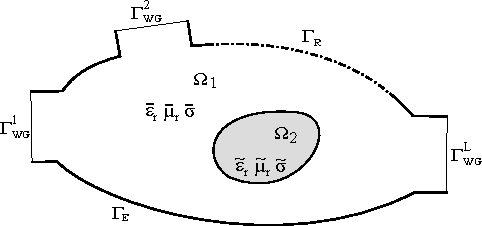
\includegraphics[width=10cm]{geometryLarge}
\caption{Generic multiport device where the total domain $\Omega$ is subdivided into linear subdomain $\Omega_1$ and a nonlinear subdomain $\Omega_2$.}
\label{fig:geometry}
\end{figure}

Given a generic multiport device (Fig.~\ref{fig:geometry}), its
domain $\Omega$, with boundary $\Gamma$, can be divided into a part $\Omega_1$ comprising only linear media, and another part $\Omega_2$ comprising all nonlinear media, with $\Omega = \Omega_1 \cup \Omega_2$ and
$\Omega_1 \cap \Omega_2 = \emptyset$.

The permittivity, the inverse of the permeability, that is the reluctivity, and the conductivity in $\Omega$ can be expressed as 
%
\begin{gather}
\epsilon_r(\mathbf{E}(\mathbf{r}),\mathbf{r}) = 
\begin{cases}
\bar{\epsilon}_r(\mathbf{r}), & \mathbf{r} \in \Omega_1,  \\
\tilde{\epsilon}_r(\mathbf{E}(\mathbf{r}), \mathbf{r}) \!=\!
\bar{\epsilon}_r(\mathbf{r}) \!+\! \mathcal{N}_\epsilon(\mathbf{E}(\mathbf{r})), & \mathbf{r} \in
\Omega_2,
\end{cases} \label{eq:epsnl}\\
\mu_r^{-1}(\mathbf{H}(\mathbf{r}),\mathbf{r}) = \nu_r(\mathbf{H}(\mathbf{r}),\mathbf{r}) = 
\begin{cases}
\bar{\nu}_r(\mathbf{r}), & \mathbf{r} \in \Omega_1, \\
\tilde{\nu}_r(\mathbf{H}(\mathbf{r}), \mathbf{r}) \!=\!
\bar{\nu}_r(\mathbf{r}) \!+\! \mathcal{N}_\nu(\mathbf{H}(\mathbf{r})), & \mathbf{r} \in
\Omega_2,
\end{cases}\label{eq:munl}\\
\sigma(\mathbf{E}(\mathbf{r}),\mathbf{r}) = 
\begin{cases}
\bar{\sigma}(\mathbf{r}), & \mathbf{r} \in \Omega_1, \\
\tilde{\sigma}(\mathbf{E}(\mathbf{r}), \mathbf{r}) \!=\!
\bar{\sigma}(\mathbf{r}) \!+\! \mathcal{N}_\sigma(\mathbf{E}(\mathbf{r})), & \mathbf{r} \in
\Omega_2,
\end{cases}\label{eq:signl}
\end{gather}

\noindent where $\mathbf{E}(\mathbf{r})$ is the electric field in the generic point
$\mathbf{r}$, $\mathbf{H}(\mathbf{r})$ is the magnetic field tightly bound to the electric field by \eqref{eq:waveeqErecH}. $\mathcal{N}_\times(\cdot)$ denotes a generic scalar operator describing the nonlinear behavior \cite{Guarnieri2010}. 

The electric field satisfies, within $\Omega$, the wave equation \eqref{eq:waveeqE}, here reported for convenience,
\begin{multline}
\nabla \times \nu_r(\mathbf{H}(\mathbf{r}),\mathbf{r}) \ \nabla \times {\mathbf{E}(\mathbf{r})} \ + j k_0 \zeta_0 \sigma(\mathbf{E}(\mathbf{r}),\mathbf{r}) \ {\mathbf{E}(\mathbf{r})} \ - k_0^2 \epsilon_r(\mathbf{E}(\mathbf{r}),\mathbf{r}) \ {\mathbf{E}(\mathbf{r})} = 0,\label{eq:waveeqEnl}
\end{multline}
\noindent where material properties are substituted by the relations \eqref{eq:epsnl}, \eqref{eq:munl} and \eqref{eq:signl}. The boundary conditions on $\Gamma$ can be any of those employed in chapter \ref{chap:FE}. For instance, in the following sections only transfinite elements will be employed on the waveports.
% $\Gamma_{12}$ corresponds to the internal boundary between subdomains $\Omega_1$ and $\Omega_2$.

The Galerkin framework applied to the problem leads to (see chapter \ref{chap:FE}) 
%
\begin{multline}
\label{eq:FEMformnl}
\int_\Omega \nabla \times \mathbf{w}_i^*(\mathbf{r}) \cdot \nu_r(\mathbf{H}(\mathbf{r}),\mathbf{r}) \nabla \times \mathbf{E}(\mathbf{r}) \ d\Omega \ + \\
 \hspace{-5cm} j k_0 \zeta_0 \int_\Omega \mathbf{w}_i^*(\mathbf{r}) \cdot \sigma(\mathbf{E}(\mathbf{r}),\mathbf{r}) \ \mathbf{E}(\mathbf{r}) \ d\Omega \ - \\
 \hspace{-3cm} k_0^2 \int_\Omega \mathbf{w}_i^*(\mathbf{r}) \cdot \epsilon_r(\mathbf{E}(\mathbf{r}),\mathbf{r}) \ \mathbf{E}(\mathbf{r}) \ d\Omega \ = \\
\int_{\Gamma} \mathbf{w}_i^*(\mathbf{r})  \times \nu_r(\mathbf{H}(\mathbf{r}),\mathbf{r}) \nabla \times {\mathbf{E}}(\mathbf{r}) \cdot \hat{\mathbf{n}} \ d\Gamma, 
\quad \forall \mathbf{w}_i(\mathbf{r}) \in \mathcal{W}_E.
\end{multline}

The multiharmonic dependence in the HBFE method is introduced by approximating the time and space dependent electric field $\mathcalb{E}(\mathbf{r},t)$ as a finite sum of harmonic components \cite{bachinger2005numerical}
%
\begin{equation} \label{eq:field}
\hat{\mathcalb{E}}(\mathbf{r}, t) = \sum^P_{p=1} \left( \mathbf{E}_{p}^{(s)}(\mathbf{r}) \sin(p
\omega_0 t) + \mathbf{E}_p^{(c)}(\mathbf{r}) \cos(p \omega_0 t) \right)
\end{equation} 

\noindent where $\omega_0$ is the fundamental angular frequency and, here and in the following, the hat over a quantity denotes its approximated value given by
the truncated Fourier series. 
$\mathbf{E}_{p}^{(s)}(\mathbf{r})$ and $\mathbf{E}_{p}^{(c)}(\mathbf{r})$ are the spatial basis functions defined as
$$
\mathbf{E}_{p}^{(s)}(\mathbf{r}) := \sum_{j=1}^{N} x_j^{(s)} \mathbf{w}_j(\mathbf{r}), \qquad \mathbf{w}_j(\mathbf{r}) \in \mathcal{W}_E,
$$ and
$$
\mathbf{E}_{p}^{(c)}(\mathbf{r}) := \sum_{j=1}^{N} x_j^{(c)} \mathbf{w}_j(\mathbf{r}), \qquad \mathbf{w}_j(\mathbf{r}) \in \mathcal{W}_E.
$$
and they expand, as in the conventional single harmonic case the field at $p\omega_0$. Hence they must individually satisfy the wave equation with $k_0 \leftarrow pk_0$.

The material properties can also be approximated as a truncated Fourier series \cite{copeland2010domain}
%
\begin{multline} \label{eq:matfourier}
\hat{{\epsilon}}_r(\mathbf{E}(\mathbf{r}), \mathbf{r}, t) = {\epsilon}_{r_0}(\mathbf{E}(\mathbf{r}),\mathbf{r}) \ + \\
\sum^{G_\epsilon}_{g=1} {\epsilon}_{r_g}^{(s)}(\mathbf{E}(\mathbf{r}),\mathbf{r}) \sin(g \omega_0 t) + \ \\ \sum^{G_\epsilon}_{g=1}  {\epsilon}_{r_g}^{(c)}(\mathbf{E}(\mathbf{r}),\mathbf{r}) \cos(g \omega_0 t),
\end{multline} 
\begin{multline} 
\hat{{\nu}}_r(\mathbf{H}(\mathbf{r}), \mathbf{r}, t) = {\nu}_{r_0}(\mathbf{H}(\mathbf{r}),\mathbf{r}) \ + \\ \sum^{G_\nu}_{g=1}  {\nu}_{r_g}^{(s)}(\mathbf{H}(\mathbf{r}),\mathbf{r}) \sin(g \omega_0 t) \ + \\
 \sum^{G_\nu}_{g=1} {\nu}_{r_g}^{(c)}(\mathbf{H}(\mathbf{r}),\mathbf{r}) \cos(g \omega_0 t),
\end{multline} 
\begin{multline} 
\hat{{\sigma}}(\mathbf{E}(\mathbf{r}), \mathbf{r}, t) = {\sigma}_{0}(\mathbf{E}(\mathbf{r}),\mathbf{r}) \ + \\
\sum^{G_\sigma}_{g=1} {\sigma}_{g}^{(s)}(\mathbf{E}(\mathbf{r}),\mathbf{r}) \sin(g \omega_0 t) \ + \\
\sum^{G_\sigma}_{g=1} {\sigma}_{g}^{(c)} (\mathbf{E}(\mathbf{r}),\mathbf{r}) \cos(g \omega_0 t),
\end{multline}
where the coefficients of the expansions are given by
\begin{equation}
\left\{
\begin{aligned} \label{eq:epsCoeffs}
{\epsilon}_{r_{0}}(\mathbf{E}(\mathbf{r}),\mathbf{r}) &= \frac{\omega_0}{2\pi}\int_0^{\frac{2\pi}{\omega_0}}
{\epsilon}_r(\mathbf{E}(\mathbf{r}),\mathbf{r}) \ dt, \\[.5cm]
{\epsilon}_{r_{g}}^{(s)}(\mathbf{E}(\mathbf{r}),\mathbf{r}) &=  \frac{\omega_0}{\pi}\int_0^{\frac{2\pi}{\omega_0}}
{\epsilon}_r(\mathbf{E}(\mathbf{r}),\mathbf{r}) \ \sin(g \omega_0 t) \ dt, \\[.5cm]
{\epsilon}_{r_{g}}^{(c)}(\mathbf{E}(\mathbf{r}),\mathbf{r}) &=  \frac{\omega_0}{\pi}\int_0^{\frac{2\pi}{\omega_0}} 
{\epsilon}_r(\mathbf{E}(\mathbf{r}),\mathbf{r}) \ \cos(g \omega_0 t) \ dt,
\end{aligned}
\right.
\end{equation}
\begin{equation}
\left\{
\begin{aligned} \label{eq:nuCoeffs}
{\nu}_{r_{0}}(\mathbf{H}(\mathbf{r}),\mathbf{r}) &=  \frac{\omega_0}{2\pi}\int_0^{\frac{2\pi}{\omega_0}}
{\nu}_r(\mathbf{H}(\mathbf{r}),\mathbf{r}) \ dt, \\
{\nu}_{r_{g}}^{(s)}(\mathbf{H}(\mathbf{r}),\mathbf{r}) &=  \frac{\omega_0}{\pi}\int_0^{\frac{2\pi}{\omega_0}}
{\nu}_r(\mathbf{H}(\mathbf{r}),\mathbf{r}) \ \sin(g \omega_0 t) \ dt, \\ 
{\nu}_{r_{g}}^{(c)}(\mathbf{H}(\mathbf{r}),\mathbf{r}) &=  \frac{\omega_0}{\pi}\int_0^{\frac{2\pi}{\omega_0}} 
{\nu}_r(\mathbf{H}(\mathbf{r}),\mathbf{r}) \ \cos(g \omega_0 t) \ dt, 
\end{aligned}
\right.
\end{equation}
\begin{equation}
\left\{
\begin{aligned} \label{eq:sigCoeffs}
{\sigma}_{0}(\mathbf{E}(\mathbf{r}),\mathbf{r}) &=  \frac{\omega_0}{2\pi}\int_0^{\frac{2\pi}{\omega_0}}
{\sigma}(\mathbf{E}(\mathbf{r}),\mathbf{r}) \ dt, \\
{\sigma}_{{g}}^{(s)}(\mathbf{E}(\mathbf{r}),\mathbf{r}) &=  \frac{\omega_0}{\pi}\int_0^{\frac{2\pi}{\omega_0}}
{\sigma}(\mathbf{E}(\mathbf{r}),\mathbf{r}) \ \sin(g \omega_0 t) \ dt, \\ 
{\sigma}_{{g}}^{(c)}(\mathbf{E}(\mathbf{r}),\mathbf{r}) &=  \frac{\omega_0}{\pi}\int_0^{\frac{2\pi}{\omega_0}} 
{\sigma}(\mathbf{E}(\mathbf{r}),\mathbf{r}) \ \cos(g \omega_0 t) \ dt.
\end{aligned}
\right.
\end{equation}

The orders of the approximations $P$ and $G_\times$ reflects on the accuracy of the solution and hence must be chosen upon appropriate energy criterion, for example retaining the part of the spectrum that have more than a prescribed portion of spectral power.

A conventional Galerkin approach, discretization of \eqref{eq:FEMformnl} 
%via \eqref{e:femexpansion}
leads to a system in the form $\mat{A}\vect{x} = \vect{b}$ with $\mat{A} \in \mathbb{C}^{N \times N}$, $\vect{x}$ and $\vect{b} \in \mathbb{C}^{N}$ (chapter \ref{chap:FE}).

In an HBFE approach, the following substitutions are performed in \eqref{eq:FEMformnl} 
\begin{gather*}
 \mathbf{E}(\mathbf{r}) \longrightarrow \hat{\mathcalb{E}}(\mathbf{r}, t), \\
 \epsilon_r(\mathbf{E}(\mathbf{r}),\mathbf{r}) \longrightarrow \hat{\epsilon}_r(\mathbf{E}(\mathbf{r}),\mathbf{r}, t),\\
\nu_r(\mathbf{H}(\mathbf{r}),\mathbf{r}) \longrightarrow \hat{\nu}_r(\mathbf{H}(\mathbf{r}),\mathbf{r}, t),\\
\sigma(\mathbf{E}(\mathbf{r}),\mathbf{r}), \longrightarrow \hat{\sigma}(\mathbf{E}(\mathbf{r}),\mathbf{r}, t).
\end{gather*}
Then, upon performing further testing with weights $\sin(q \omega t)$ or $\cos(q \omega t)$, $q = 1 \dots P$, and integrating over the time period of the fundamental $\left [ 0,\frac{2\pi}{\omega} \right )$,  a large linear system is obtained which has formally the same structure as a conventional finite element system but multiple matrices $\mat{A}$ and vectors $ \vect{x}$ and $\vect{b}$ are assembled depending on the harmonic of testing. The final system matrix can hence be represented as
%
\begin{equation}\label{eq:HBfemmn}
\begin{bmatrix}
\mat{A}^{(1s1s)} & \mat{A}^{(1s1c)} & \ldots &  \mat{A}^{(1sPc)} \\
\mat{A}^{(1c1s)} & \mat{A}^{(1c1c)} & \ldots &  \mat{A}^{(1cPc)} \\
\vdots & \vdots & \ddots & \vdots \\
\mat{A}^{(Pc1s)} & \mat{A}^{(Pc1c)} & \ldots &  \mat{A}^{(PcPc)}
\end{bmatrix}
\begin{bmatrix}
\vect{x}^{(1s)} \\
\vect{x}^{(1c)} \\
\vdots \\
\vect{x}^{(Pc)}
\end{bmatrix}
=
\begin{bmatrix}
\vect{b}^{(1s)}\\
\vect{b}^{(1c)}\\
\vdots\\
\vect{b}^{(Pc)}
\end{bmatrix}.
\end{equation}

\noindent The superscripts $(q[s|c])$ and $(p[s|c])$ indicates that the corresponding
entry was computed by testing \eqref{eq:FEMformnl} with $[\sin(q \omega t) | \cos(q \omega t)]$ while the corresponding harmonic basis of \eqref{eq:field}
was $[\sin(p \omega t) | \cos(p \omega t)]$. Harmonic coupling, which clearly worsen the system matrix sparsity, only occurs within elements pertaining to nonlinear material solids, for instance, off-diagonal sub-matrices of \eqref{eq:HBfemmn} vanish within linear materials.

The nonlinearity is finally handled via a relaxed iteration. As a starting point a null electric field $\vect{x}^0$ is assumed, computing the pertinent system matrix $\mat{A_{([x]^0)}}$ and known term $\vect{b_{([x]^0)}}$ and solving the system $\mat{A_{([x]^0)}} \vect{x}^1 = \vect{b_{([x]^0)}}$. The newly computed field $\vect{x}^1$ can now be used to update system matrix and known term and perform the following relaxed iteration:
% %
\begin{equation} \label{eq:lastLinearSystem}
 \mat{A_{(\gamma \vect{x}^{i-1} + (1-\gamma) \vect{x}^{i-2})}} \vect{x}^{i} = \vect{b_{(\gamma \vect{x}^{i-1} + (1-\gamma) \vect{x}^{i-2})}},
\end{equation}

\noindent with $i \geq 2$ and $\gamma\in(0,1]$. $\gamma=1$ gives the standard Picard iteration \cite{Guarnieri2010}, while low $\gamma$ values damps the oscillations
which may arise with highly nonlinear materials or high intensity impressed
fields at the cost of a slower convergence \cite{Silvester1997}. The process 
is repeated until the relative error between the updated solution
and the previous one, in the sense of the Euclidean norm, is less than a
prescribed value $\tau$, that is
$$ \frac{\Vert\vect{x}^{i}-\vect{x}^{i-1} \Vert_2}{\Vert\vect{x}^{i}\Vert_2} < \tau.$$

\section{Harmonic testing generalities}

The multi-harmonic testing can straightforwardly exploit the orthogonality between sine and cosine function defined as
%
\begin{eqnarray*}
\frac{\omega_0}{\pi}\int_{0}^{\frac{2\pi}{\omega_0}} \cos(m \omega_0 t) \ \cos(n \omega_0 t) \ dt &= &\delta_{mn},\\
\frac{\omega_0}{\pi}\int_{0}^{\frac{2\pi}{\omega_0}} \sin(m \omega_0 t) \ \sin(n \omega_0 t) \ dt &= &\delta_{mn},\\
\frac{\omega_0}{\pi}\int_{0}^{\frac{2\pi}{\omega_0}} \sin(m \omega_0 t) \ \cos(n \omega_0 t) \ dt &= &0,
\end{eqnarray*}
%
\noindent and for the constant terms in materials characteristics we have
\begin{eqnarray*}
\frac{\omega_0}{2\pi}\int_{0}^{\frac{2\pi}{\omega_0}} \cos(n \omega_0 t) \ dt &= & 1,\\
\frac{\omega_0}{2\pi}\int_{0}^{\frac{2\pi}{\omega_0}} \sin(n \omega_0 t) \ dt &= & 1,
\end{eqnarray*}
%
\noindent where $m \neq 0$, $n \neq 0$ and $\delta_{mn}$ is the Kronecker delta. Once the material properties expansion coefficients are computed, it might seem that the testing of \eqref{eq:FEMformnl} on the time period involves more than two trigonometric functions. It is possible to compute such testing integrals simply upon exploiting the following relations between the products of trigonometric functions
\begin{gather}
\cos (m \omega t) \cos(n \omega t) = \frac{1}{2} \cos ((m-n) \omega t ) + \frac{1}{2}  \cos((m+n) \omega t), \\
\sin (m \omega t) \sin(n \omega t) = \frac{1}{2} \cos ((m-n) \omega t ) - \frac{1}{2}  \cos((m+n) \omega t), \\
\sin (m \omega t) \cos(n \omega t) = \frac{1}{2} \sin ((m-n) \omega t ) + \frac{1}{2}  \sin((m+n) \omega t),
\end{gather}
\noindent hence splitting them into integrals that involve only two trigonometric functions.

All the testings on material properties can be either precomputed analytically, up to some prescribed orders, or numerically by the use of the fast fourier transform (FFT) \cite{frigo2005design}. The FFT is an efficient algorithm that implements the discrete Fourier transform, defined as
\begin{equation}
X_q = \sum_{k=0}^{N-1} x_k \exp{-j \frac{2\pi}{N} k q}, \qquad q=0,1,\ldots,N-1.
\end{equation}
\noindent When $x_k$ is a sequence of $N$ samples of $\hat{\epsilon}_r(\mathbf{E}(\mathbf{r}),\mathbf{r}, t)$, $\hat{\nu}_r(\mathbf{H}(\mathbf{r}),\mathbf{r}, t)$ or $\hat{\sigma}(\mathbf{E}(\mathbf{r}),\mathbf{r}, t)$ within the period $[0, \frac{2\pi}{\omega_0})$, then $X_q$ correspond to the expansion coefficients at the given normalized frequencies $q = \frac{g \omega_0}{\omega_0}$. Of course, one must use Euler formulas 
\begin{gather}
\cos (nt) = \frac{\exp{jnt} + \exp{-jnt}}{2},\\
\sin (nt) = \frac{\exp{jnt} - \exp{-jnt}}{2j},\\
\exp {jnt} = \cos(nt) + j \sin(nt),
\end{gather}
\noindent before and after the FFT and changing the phase where necessary to recover the proper values.

As will be shown in the intermodulation products example, $p, q$ and $g$ do not necessarily need to be integers. In fact, when considering multiple signals feeding a nonlinear device, these generate higher-order harmonics at multiples of the sum or difference between the impinging signals frequencies. Hence, for the necessary computational accuracy, the largest sampling period has to be considered in an FFT testing algorithm, and this is given by the largest common divisor between all the impinging signals.

\section{Transverse magnetic field formulation}

Let us assume the electric field $\mathbf{E}$ to be only $\hat{\mathbf{z}}$-directed such that $\mathbf{E} = E_z \hat{\mathbf{z}}$. Both fields and material properties are assumed not to vary along the $\hat{\mathbf{z}}$ direction and hence $E_z = E_z(x,y)$ and the magnetic field will have only transverse components, that is $H_x(x,y)$ and $H_y(x,y)$. Then the wave equation 
$$\nabla \times \dyad{\nu}_r \ \nabla \times {\mathbf{E}} + j k_0 \zeta_0 \dyad{\sigma} \ {\mathbf{E}} - k_0^2 \dyad{\epsilon}_r \ {\mathbf{E}} = 0,$$
\noindent becomes
\begin{equation}
\label{eq:helmholtz}
\nabla \cdot \dyad{\nu}_r \ \nabla {E_z} - j k_0 \zeta_0 \dyad{\sigma} \ {E_z} + k_0^2 \dyad{\epsilon}_r \ {E_z} = 0.
\end{equation}
\noindent In fact, we have
$$\nabla \times \dyad{\nu}_r \nabla \times E_z \hat{\mathbf{z}} = \nabla \times  (-\hat{\mathbf{z}} \times \dyad{\nu}_r \nabla E_z), $$
\noindent and by the use of the relation \cite{van2007electromagnetic} $\nabla \times  (\hat{\mathbf{z}} \times \mathbf{v}) = \hat{\mathbf{z}} \nabla \cdot \mathbf{v} - \frac{\partial \mathbf{v}}{\partial z}$ and remembering that $E_z(x,y)$ is independent on the $z$ variable, we have
$$\nabla \times (-\hat{\mathbf{z}} \times \dyad{\nu}_r \nabla E_z) = -\hat{\mathbf{z}} \nabla \cdot \dyad{\nu}_r \nabla E_z - \underbrace{\frac{\partial \dyad{\nu}_r \nabla E_z}{\partial z}}_{= 0}.$$
\noindent Finally we achieve
$$
-\hat{\mathbf{z}} \nabla \cdot \dyad{\nu}_r \ \nabla {E_z} + j k_0 \zeta_0 \dyad{\sigma} \ {E_z \hat{\mathbf{z}}} - k_0^2 \dyad{\epsilon}_r \ {E_z \hat{\mathbf{z}}} = 0.
$$
\noindent which can be written as \eqref{eq:helmholtz} upon removing the $\hat{\mathbf{z}}$ and multiplying by $-1$ all the terms of the equation. The field $E_z$ can be expanded with scalar basis functions $\phi \in \mathcal{V}(\Omega_h) := \{ \phi \in  \} \subset \mathcal{H}^1(\Omega, \Gamma_E)$ such that
$$E_{z} = \sum_{j=1}^{N_z} x_{z,j} \phi_j.$$
\noindent Galerkin projection leads to the following weak form
\begin{multline}
\int_\Omega \nabla \phi_i^* \cdot \dyad{\nu}_r \ \nabla {E_z} \ d\Omega + j k_0 \zeta_0 \int_\Omega \phi_i^* \dyad{\sigma} \ {E_z} \ d\Omega \ - \ \\ k_0^2 \int_\Omega \phi_i^* \dyad{\epsilon}_r \ {E_z} d\Omega = \int_\Gamma \phi_i^* \dyad{\nu}_r \ \nabla {E_z} \cdot \hat{\mathbf{n}} \ d\Gamma.
\end{multline}
\noindent where the vector identity $A \nabla \cdot \mathbf{B} = \nabla \cdot (A \mathbf{B} ) - \nabla A \cdot \mathbf{B}$ and Gauss' theorem have been exploited \cite{van2007electromagnetic}. $\hat{\mathbf{n}}$ is the outwardly directed normal unit vector.

Due to the field homogeneity along the $\hat{\mathbf{z}}$ direction, only a few components of materials tensors will contribute to the equation, for instance
\begin{gather}
\dyad{\nu}_r = 
\begin{bmatrix}
\nu_{r,\mathbf{x}\mathbf{x}} & \nu_{r,\mathbf{x}\mathbf{y}}\\
\nu_{r,\mathbf{y}\mathbf{x}} & \nu_{r,\mathbf{y}\mathbf{y}}
\end{bmatrix} = \begin{bmatrix}
\mu_{r,\mathbf{x}\mathbf{x}} & \mu_{r,\mathbf{x}\mathbf{y}}\\
\mu_{r,\mathbf{y}\mathbf{x}} & \mu_{r,\mathbf{y}\mathbf{y}}
\end{bmatrix}^{-1},\\
\dyad{\sigma} = \sigma_{\mathbf{z}\mathbf{z}},\\
\dyad{\epsilon}_r = \epsilon_{r,\mathbf{z}\mathbf{z}}.
\end{gather}

All the considerations made in chapter \ref{chap:FE} can be applied on $\Gamma$ integrals upon imposing the previous condition on the electric field. In particular, we will consider the waveports segments of figure \ref{fig:geometry} (as in 2D problem) with impinging $\mathrm{TE}_{m0}$ modes with $m \in \mathbb{N}^+$, hence respecting the $\mathbf{E} = E_z \hat{\mathbf{z}}$ condition. Also here, the modal distributions can be computed either analytically \cite{pelosi2009quick} or numerically by solving the transverse-longitudinal eigenvalue one-dimensional problem analogously to what is done in chapter \ref{chap:FE} for a two-dimensional problem.

\section{Numerical tests}

Here follows three tests performed to illustrate the performances of the HBFE method for the wave equation.

\subsection{Millimeter-wave bandpass filter with nonlinear dielectrics}

\begin{figure}[ht!]
\centering
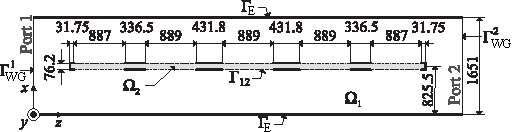
\includegraphics[width=13.4cm]{bilat}
\caption{Cross section (H-plane) of a passband filter realized
by placing on the E-plane a dielectric slab partially metalized on both sides
(slab is shown in light grey; metal strips - uniform along $y$ are shown as
thick black lines) in a WR6 rectangular waveguide. Measures are given in $\mu{m}$.}
\label{fig:bilat}
\end{figure}

The millimeter-wave passband filter in WR6 (1651x825.5~$\mu$m) rectangular 
waveguide, initially presented in chapter \ref{chap:FE} with a full-wave formulation is here analyzed with a transverse magnetic 2D formulation \cite{bui1984broad}. 
The filter, uniform along $y$ axis, is realized by placing on the E-plane a 
dielectric slab partially metalized on both sides as shown by the H-plane cross
section of Fig.~\ref{fig:bilat}. All conductors are considered perfect. $\mu_r = 1$ and $\sigma = 0$ everywhere in $\Omega$.
The dielectric, enclosed in $\Omega_2$, presents a Kerr-type nonlinearity of
such that \cite{Guarnieri2010}
%, Ma1997}
\begin{equation}
\tilde{\epsilon}_r(\vec{E}(\vec{r}), \vec{r}) = \bar{\epsilon}_r(\vec{r}) + 
\alpha_2 \ |\vec{E}(\vec{r})|^2, \qquad \vec{r} \in \Omega_2
\end{equation}
\noindent where $\bar{\epsilon}_r(\vec{r}) = 2.1$ and 
$\alpha_2~=~1.625~10^{-10}~{\frac{\mathrm{m}^2}{\mathrm{kV}^2}}$.
%is chosen as \cite{Ma1997}. 

The Kerr-like behavior of the permittivity induces the generation of odd order harmonics, thus 
even ones can been neglected. For the relaxed
iteration stop criterion, $\tau = 10^{-6}$ has been chosen.
The continuity of the field at the ports is imposed through a modal expansion 
exploiting only $\mathrm{TE}_{m0}$ modes, $m = 2n+1$, $n=1,\ldots,4$, even $m$
modes being absent for the E-plane symmetry of the filter.  
The excitation is a $\mathrm{TE}_{10}$ mode at fundamental frequency impinging at
Port 1 with maximum field amplitude $E_ i$. The 
waveguide discontinuity represented by the filter transfers power to higher order
modes, which may result to be guided at higher harmonic frequencies.
Furthermore, as a sinusoidal excitation is chosen, only $\sin(p \omega t)$ 
related coefficients are retained.
Due to H-plane uniformity, the problem can be treated as two-dimensional \cite{pelosi2009quick}.
First order nodal elements are used and the discretization leads to 2473
degrees of freedom, 80 of which belong to the nonlinear subdomain $\Omega_2$, 
314 to the boundaries and 2079 to the linear subdomain $\Omega_1$. Such a fine
discretization is necessary to obtain a good approximation of the field up to 
the $5^\mathrm{th}$ harmonic.
%
\begin{figure}[!ht]
\centering
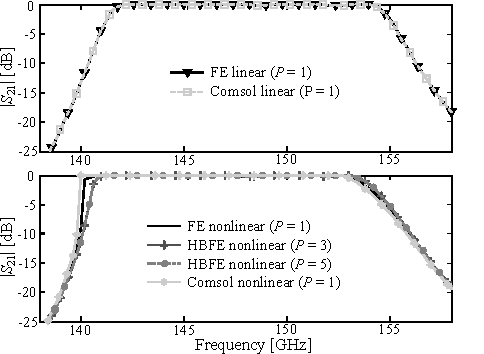
\includegraphics[width=12cm]{spectrumNHarm}
\caption{$\mathrm{TE}_{10}$ spectral response for linear (top) and nonlinear 
(bottom) permittivity with $E_i = 10$~$\frac{\mathrm{kV}}{\mathrm{m}}$. The results are compared with Comsol
RF module linear and nonlinear solutions.}
\label{fig:spectrumNHarm}
\end{figure}

As a first analysis, the effect of the total number of harmonics $P$
retained on the filter's spectral response is investigated
(Fig.~\ref{fig:spectrumNHarm}). For an incident field amplitude $E_i = 10$~${\frac{\mathrm{kV}}{\mathrm{m}}}$, the Picard iteration proved to converge. Equal mesh and parameters have been used to conduct a \mbox{2D} finite element (single harmonic) analysis with Comsol RF Module \cite{ComsolRF}. Being the nonlinear loop tackled differently (Comsol uses Newton algorithm), perfect matching in the spectral response is not obtained as for the linear permittivity case ($\alpha_2 = 0$).
It is evident from Fig.~\ref{fig:spectrumNHarm} that including 
the $3^\mathrm{rd}$ harmonic is crucial for proper evaluation of the device
bandwidth.

The electric field distribution at 146~GHz, 438~GHz and 730~GHz are shown in Fig.~\ref{fig:Fields}. As higher-order harmonics are generated by the fundamental field flowing through nonlinear parts of the device, the related fields will be, also for passivity concerns, of various orders of magnitude lower.

\begin{figure}[!ht]
\centering
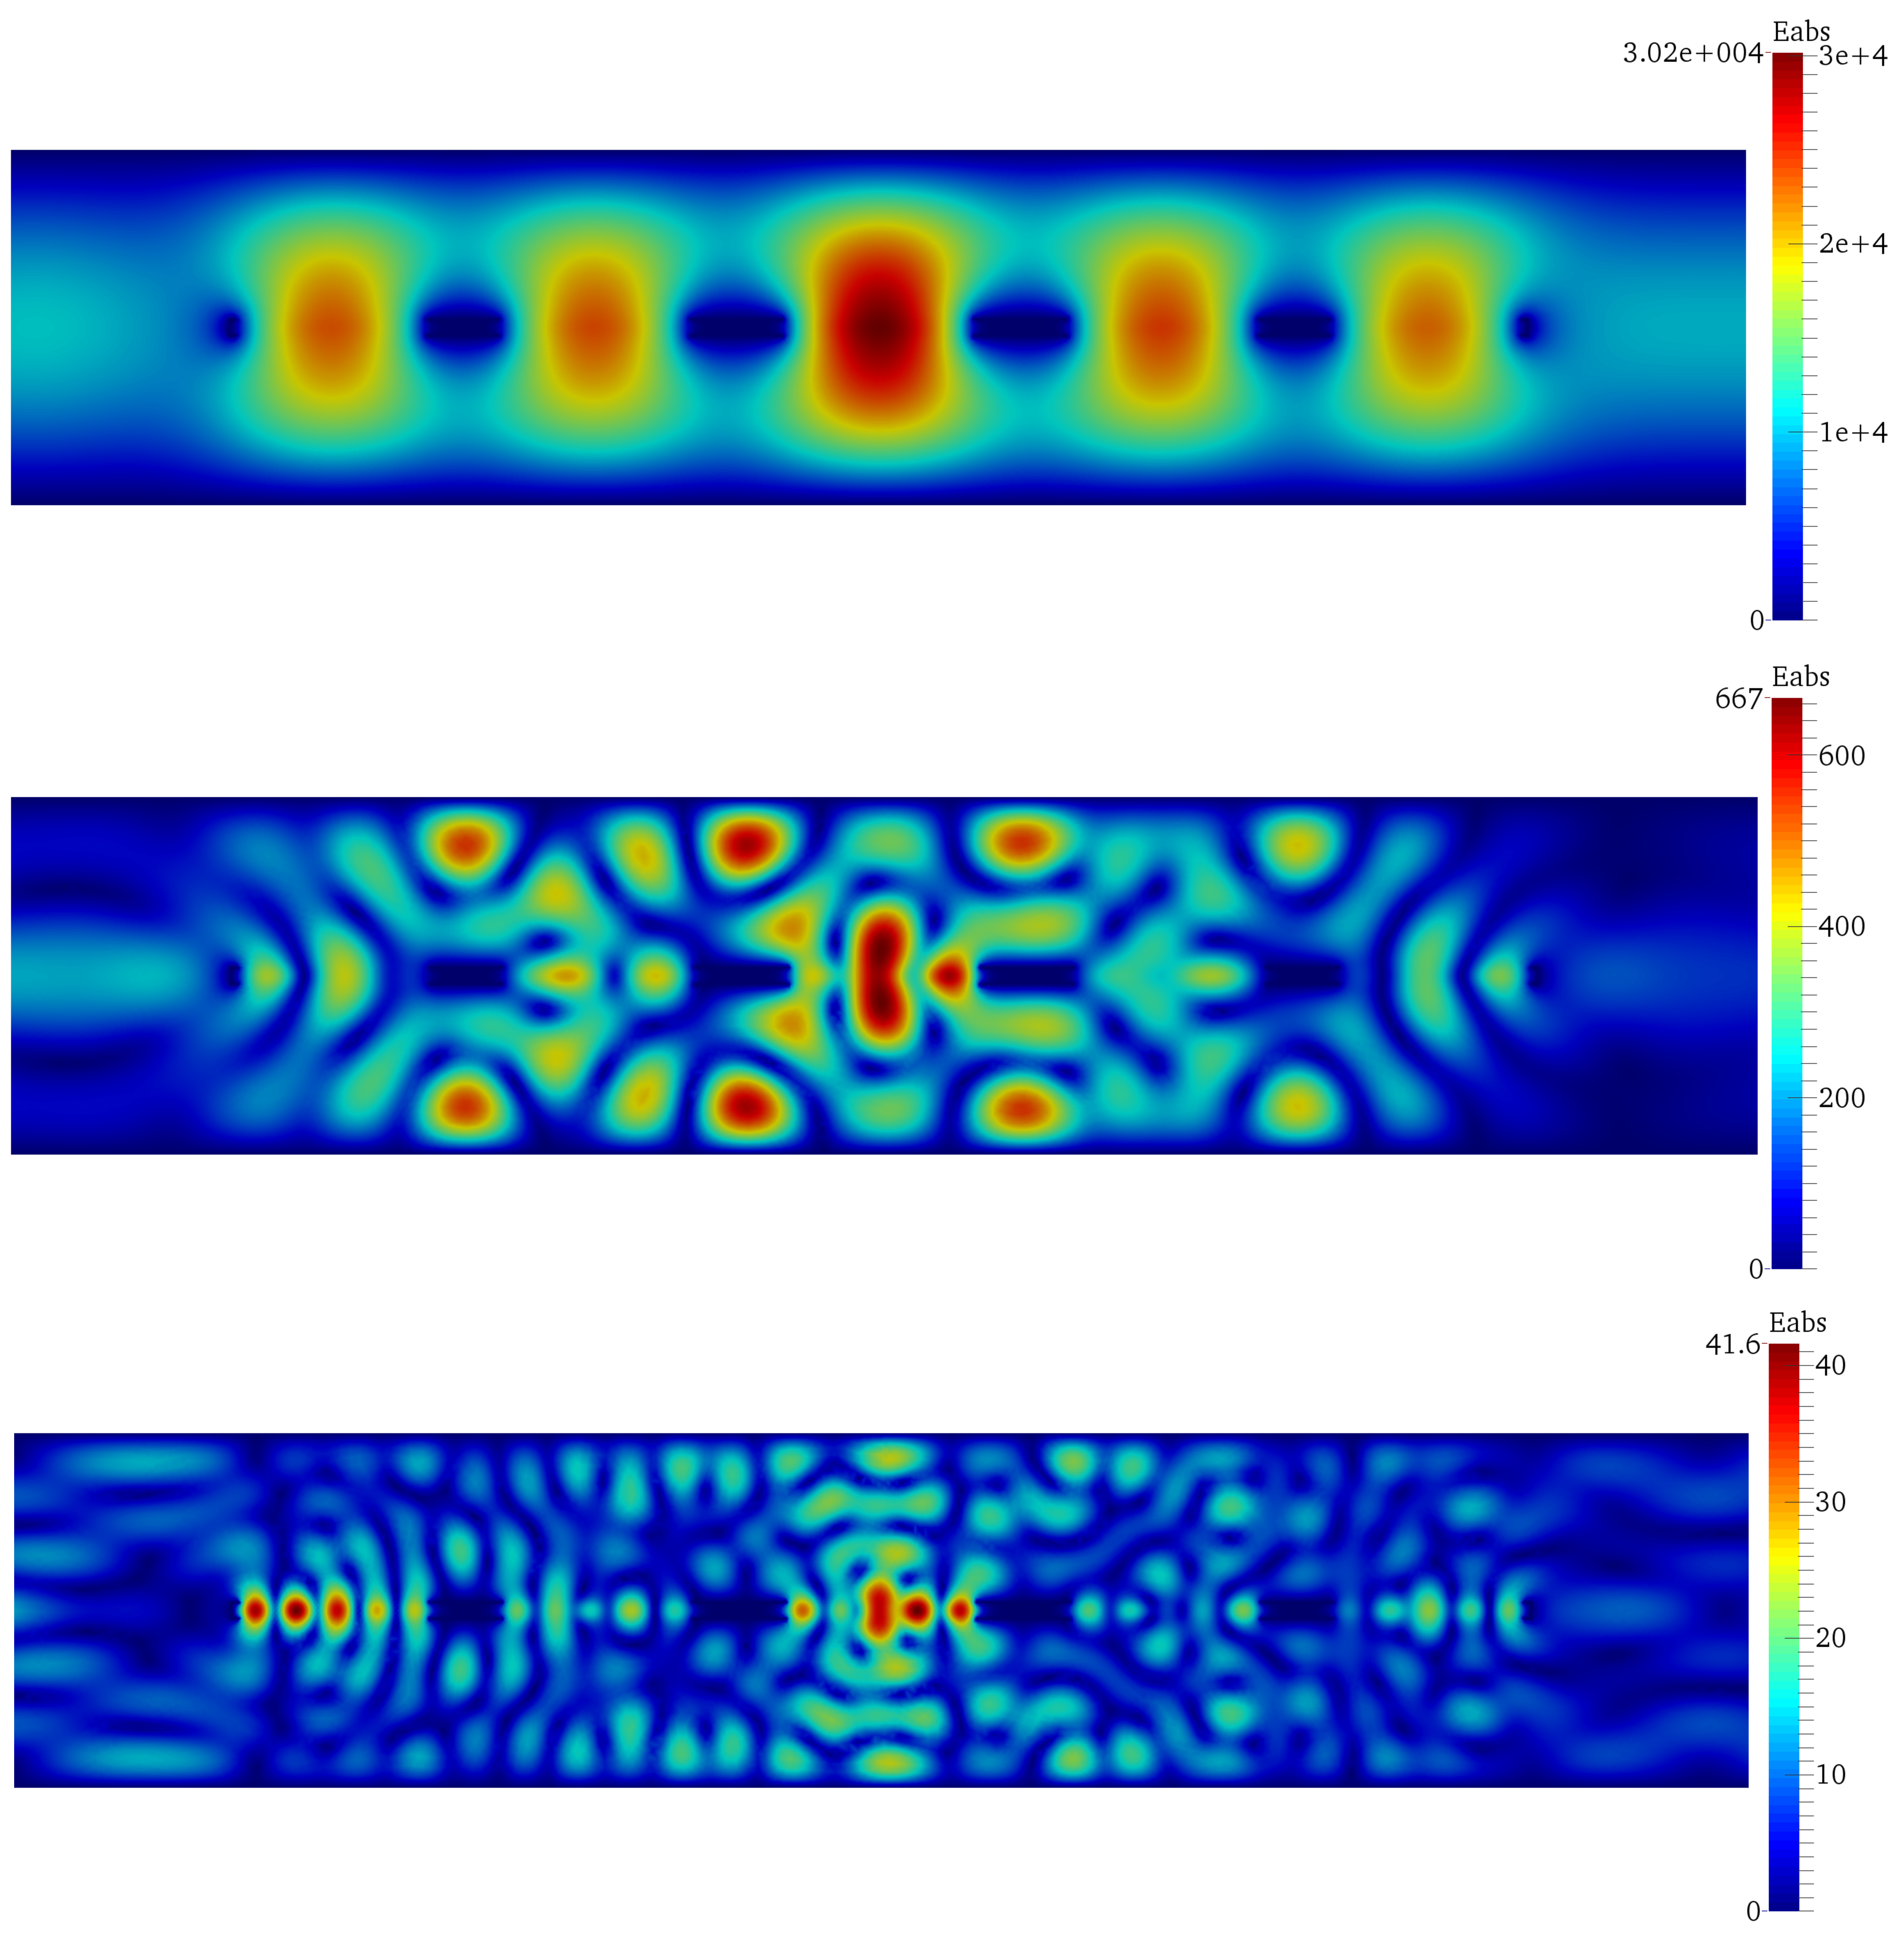
\includegraphics[width=13.4cm]{FieldsCol}
\caption{$|\mathrm{E}_y|$ distribution within the filter at fundamental 
($f_0 =$ 146 ~GHz), $3^\mathrm{rd}$ and $5^\mathrm{th}$ order harmonics 
($\mathrm{E_i = 10 ~{\frac{\mathrm{kV}}{\mathrm{m}}}}$).}
\label{fig:Fields}
\end{figure}

\begin{figure}[!ht]
\centering
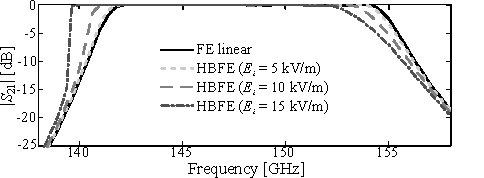
\includegraphics[width=12cm]{spectrumS21b}
\caption{$|S_{21}|$ of the nonlinear filter for
several values of $E_i$ compared to the linear case. Field is approximated
up to the $5^\mathrm{th}$ harmonic.}
\label{fig:spectrum}
\end{figure}

To gain better insight, simulations have
been repeated with $E_i=5$~${\frac{\mathrm{kV}}{\mathrm{m}}}$ and $E_i=15$~${\frac{\mathrm{kV}}{\mathrm{m}}}$, for $P=5$. 
The results compared to those of a linear device are shown in Fig.~\ref{fig:spectrum}. 
There is an evident shift of the band 
towards lower frequencies as higher power densities are involved, which agrees 
to \cite{Yatsyk2006}. Furthermore the $E_i=15$~${\frac{\mathrm{kV}}{\mathrm{m}}}$ did not 
converge with Picard iteration and required a relaxed $\gamma = 0.1$ iteration.
% In this case, the abrupt variation of $|S_{21}|$ around $139.5$~GHz points out 
% that $P=5$ is not sufficient to accurately analyze the device.
% Indeed, the power associated to harmonics grows as the incident field 
% increases as shown in Fig.~\ref{fig:harmSpectrum}. 
% \st{but a finer mesh would be necessary to allow for higher $P$ values.}
% \begin{figure}[!t]
% \centering
% 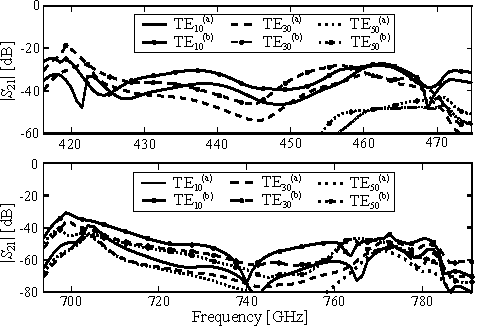
\includegraphics{harmSpectrum}
% \caption{Spectral responses at $3^\mathrm{rd}$ (top) and $5^\mathrm{th}$ 
% (bottom) harmonics
% for scattered modes (Incident $\mathrm{TE}_{10}$ with (a) $E_i = 10$~kV/m;
% (b) $E_i = 15$~kV/m.}
% \label{fig:harmSpectrum}
% \end{figure}

Analysis of the spectral response convergence is performed computing the relative
error, in Euclidean norm sense, all over the device bandwidth while increasing 
the order of HBFE system such that
\begin{equation} \label{eq:convError}
	\mathrm{error}(P=p) = \frac{\| |S_{21}|^{p} - |S_{21}|^{p-2}\|_2}
	{\| |S_{21}|^{p-2}\|_2} 
\end{equation}
\noindent with $p = 2n+1$, $n=1,\ldots,5$. Results (Fig.~\ref{fig:convergence})
show faster convergence for low intensity impinging fields.

\begin{figure}[!ht]
\centering
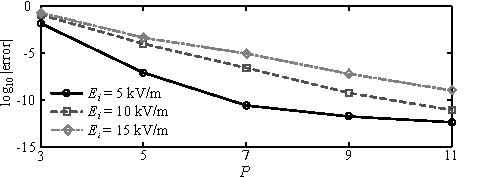
\includegraphics[width=12cm]{convergence}
\caption{
Relative error of the spectrum at fundamental frequency for various $E_i$ values.}
\label{fig:convergence}
\end{figure}

To enhance the computational efficiency, a Schur complement based domain decomposition approach is here proposed \cite{Guarnieri2010,Guarnieri2009}. The multiharmonic unknowns vector $[x]$ defined by the HBFE method over $\Omega$ can be split into two vectors $[x_{1}]$ and $[x_{2}]$ containing the unknowns belonging
to interior points in $\Omega_1$ and $\Omega_2$, respectively. Unknowns
belonging to the boundaries $\Gamma\cup\Gamma_{12}$ are placed in a third
vector $[x_{\Gamma}]$. The HBFE system can then be recast in :
%
\begin{equation}\label{eq:DD}
\begin{bmatrix}
 [A_{11}] &  0  &  [A_{1\Gamma_1}] \\
 0  &  [A_{22}]^{i-1} & [A_{2 \Gamma_2}]^{i-1} \\
 [A_{\Gamma_1 1}] & [A_{\Gamma_2 2}]^{i-1} & [A_{\Gamma \Gamma}]^{i-1}
\end{bmatrix}
\begin{bmatrix}
{[x_{1}]^{i}} \\
{[x_{2}]^{i}} \\
{[x_{\Gamma}]^{i}}
\end{bmatrix} 
=
\begin{bmatrix}
{[b_{1}]} \\
{[b_{2}]}^{i-1} \\
{[b_{\Gamma}]}^{i-1}
\end{bmatrix} 
\end{equation}

\noindent where $[A_{11}]$ contains the HBFE coefficients of the linear system
related to the unknowns $[x_{1}]$, with
null harmonic coupling coefficients, while $[A_{22}]$ contains coefficients for
the nonlinear subdomain $\Omega_2$. ${[A_{\Gamma_\times \times}]}$ and ${[A_{ \times \Gamma_\times}]}$
represent couplings between interior unknowns and 
boundary unknowns collected in $[x_\Gamma]$. 
By using the Schur complement concept, the boundary unknowns $[x_\Gamma]^{i}$ of
\eqref{eq:DD}, and hence the generalized scattering matrix of the device, can be retrieved \cite{Guarnieri2010, Guarnieri2009}.
Hence, in order to solve the HBDDFE system,
every single submatrix is assembled at first sight, then, within the iteration
loop, only the submatrices related to $\Omega_2$ and $\Gamma_{12}$ are to be
updated. The efficiency of this 
DD technique relies on the fragmentation of the
matrices and the subsequent computation of partial solutions. When the number
of coefficients related to the nonlinear media is small, noticeable
improvements can be achieved.

\begin{figure}[!ht]
\centering
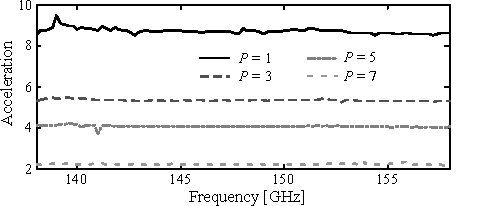
\includegraphics[width=11cm]{acceleration}
\caption{Acceleration spectrum obtained for an HBFE system of several harmonic
orders. The computations are made for $E_i = 15$~${\frac{\mathrm{kV}}{\mathrm{m}}}$~($\gamma = 0.1$).}
\label{fig:acceleration}
\end{figure}

The efficiency of the DD technique can be
assessed by its acceleration,
$$\text{Acceleration} = \frac{\text{HBFE time}}{\text{HBDDFE time}},$$
\noindent that is the ratio between time for a full domain
computation - inclusive of nonlinear iterations - and the corresponding DD
computation (assembly and solve) \cite{Guarnieri2010}. Fig.~\ref{fig:acceleration} presents the acceleration for each frequency point, and for different values of $P$ at  $E_i = 10~{\frac{\mathrm{kV}}{\mathrm{m}}}$. 

In general, higher order HBDDFE systems have lower acceleration, since the
matrices dimensions related to nonlinear media increase. With a
$P=3$ system, the acceleration varies in the range [2.51,
9.15], averaging to 4.18, and leading to an HBDDFE solution in 24\% of the
time required by a full domain HBFE solution.

\subsection{Microwave circulator intermodulation products}


The test case of a H-plane circulator in rectangular waveguide constituted by a Y-junction with a magnetized ferrite post is presented \cite{koshiba1986finite}. The circulator comprises three WR90 (cross-section dimensions $a$=22.86~mm and $b$=10.16~mm) waveguide sections of length $l$=33.4~mm joined forming a 120\textdegree~angle one with each other in a Y shape and a magnetized ferrite post of height $b$, hence spanning the whole device height. The post is an equilateral triangular prism of base side $d$=7.80~mm, placed at the center of the junction as sketched in Fig. \ref{fig:Koshiba} and it is magnetized along $\hat{\mathbf{z}}$.

\begin{figure}[!ht]
\centering
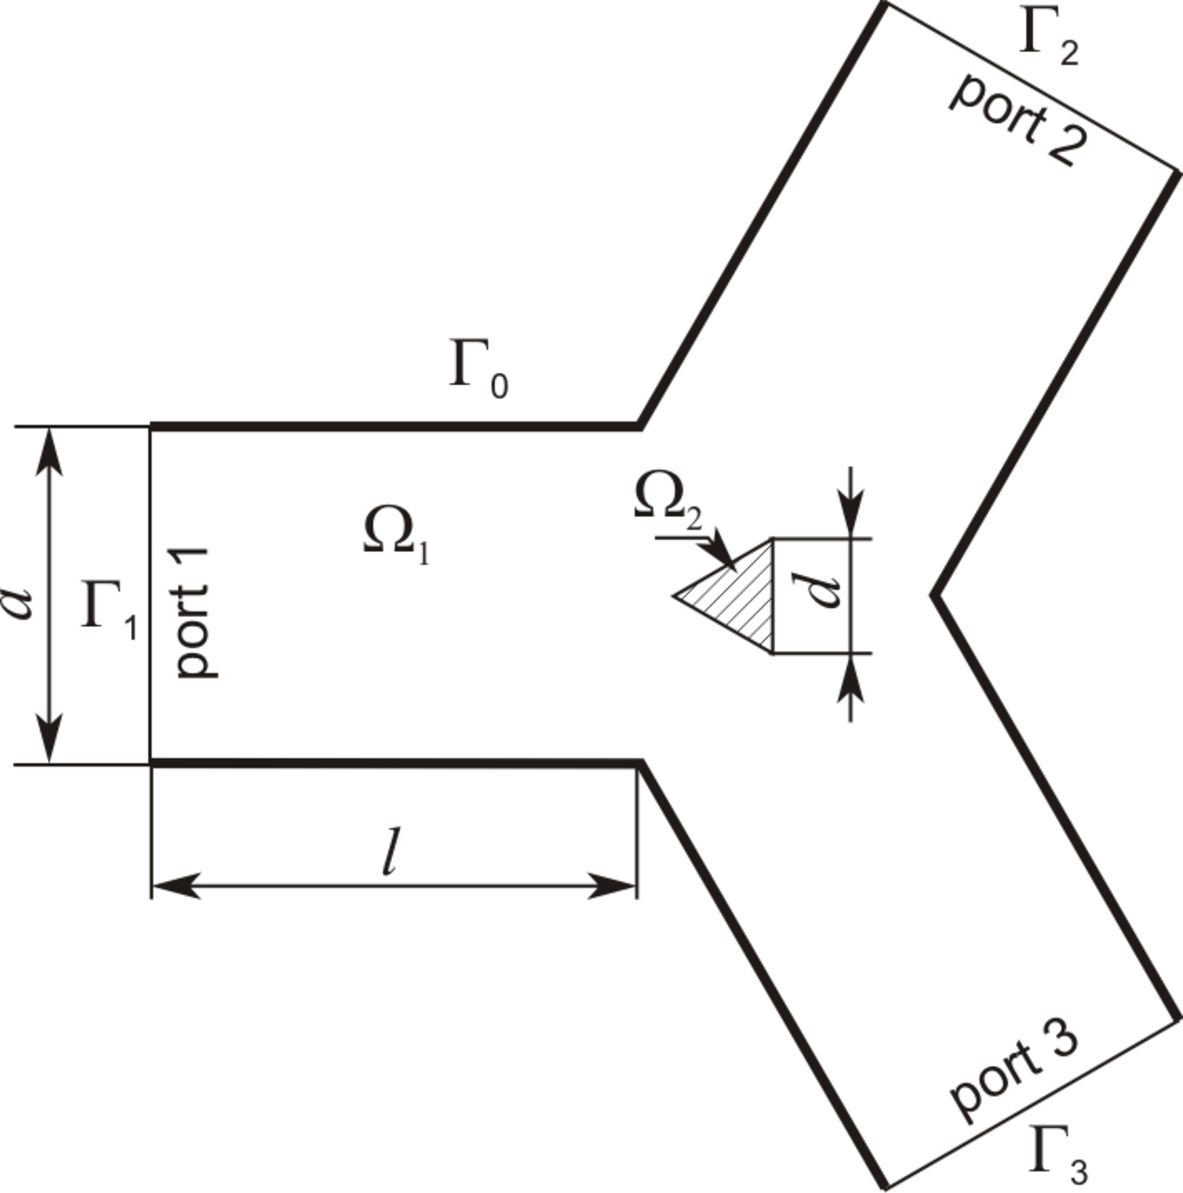
\includegraphics[width=8cm]{Koshiba}
\caption{Geometry layout of the ferrite circulator. The two domains $\Omega_1$ and $\Omega_2$, respectively corresponding to linear and nonlinear domains, are shown.}
\label{fig:Koshiba}
\end{figure}
 
While the most of the device, $\Omega_1$, is in air ($\bar{\epsilon}_r = \bar{\mu}_r = 1$), the post, $\Omega_2$, is made of a nonlinear magnetized ferrite. In \cite{koshiba1986finite} and in many other papers, the ferrite is considered linear and characterized by: 
\begin{gather}
\label{eq:ferrite}
\dyad{\mu}_r = 
\begin{bmatrix}
\mu_r& j\kappa_r\\
-j\kappa_r& \mu_r
\end{bmatrix},\\
\dyad{\epsilon}_r = \epsilon_r,
\end{gather}
%
\noindent with, as in the standard linear approach in which only the static (DC) external impressed magnetic field is considered and the harmonic (AC) signal neglected:
\begin{gather}
\label{eq:lin}
\mu_r = 1 + \frac{(\omega_0 + j\omega\alpha)\omega_m}{(\omega_0 + j\omega\alpha)^2-\omega^2}, \quad
\kappa_r = \frac{\omega\omega_m}{(\omega_0 + j\omega\alpha)^2-\omega^2},
\end{gather}
%
\noindent being $\omega_0 = \gamma H_i$, $\omega_m = \gamma M_s$, $\alpha = \gamma \frac{\Delta H}{2\omega}$; and being $H_i$ the external DC magnetic impressed field, uniform along the out of plane direction, $M_s$ the saturation magnetization,  $\Delta H$ the resonance linewidth and $\gamma$ the gyromagnetic ratio. In the following the values considered will be: $\gamma = 1.76~10^{7}~ \frac{\mathrm{C}}{\mathrm{kg}}$, $H_i = 200~\mathrm{G}$, $M_s = 1317~\mathrm{Oe}$, $\Delta H = 135~\mathrm{Oe \cdot s}$ and $\epsilon_r = 11.7$ as reported in \cite{koshiba1986finite}.

Relation \eqref{eq:ferrite} still holds for non-linear ferrites if the AC magnetic field is not neglected with respect to the external DC magnetic field. In this case $\mathbf{H} = H_i \hat{\mathbf{z}} + \mathbf{H}_\mathrm{AC}$ and $\mathbf{M} = M_s \hat{\mathbf{z}} + \mathbf{M}_\mathrm{AC}$, upon derivation from the macroscopic equation of motion for large signals and assumption of the $\hat{\mathbf{z}}$-directed components of the AC field to be neglectable, \eqref{eq:lin} are replaced by:
%
\begin{gather}
\label{eq:nl1}
\mu_r = 1 + \frac{(\omega_0 + j\omega\alpha)\omega_m}{(\omega_0 + j\omega\alpha)^2 + (\gamma H_x)^2+ (\gamma H_y)^2 -\omega^2}, \\
\label{eq:nl2}
\kappa_r = \frac{\omega\omega_m}{(\omega_0 + j\omega\alpha)^2 + (\gamma H_x)^2+ (\gamma H_y)^2-\omega^2},
\end{gather}
%
\noindent being $H_x$ and $H_y$ the two components, on the H-plane, of the AC magnetic field.

The analysis is first conducted assuming small signals impinging on Port 1 ($\Gamma_1$), hence with linear permeability tensor. The resulting spectral response is given in Fig. \ref{fig:circresplin}, and it matches the one reported by \cite{koshiba1986finite}. Figure \ref{fig:linfield} reports the corresponding fieldmap for a 9~GHz signal.

\begin{figure}[!ht]
\centering
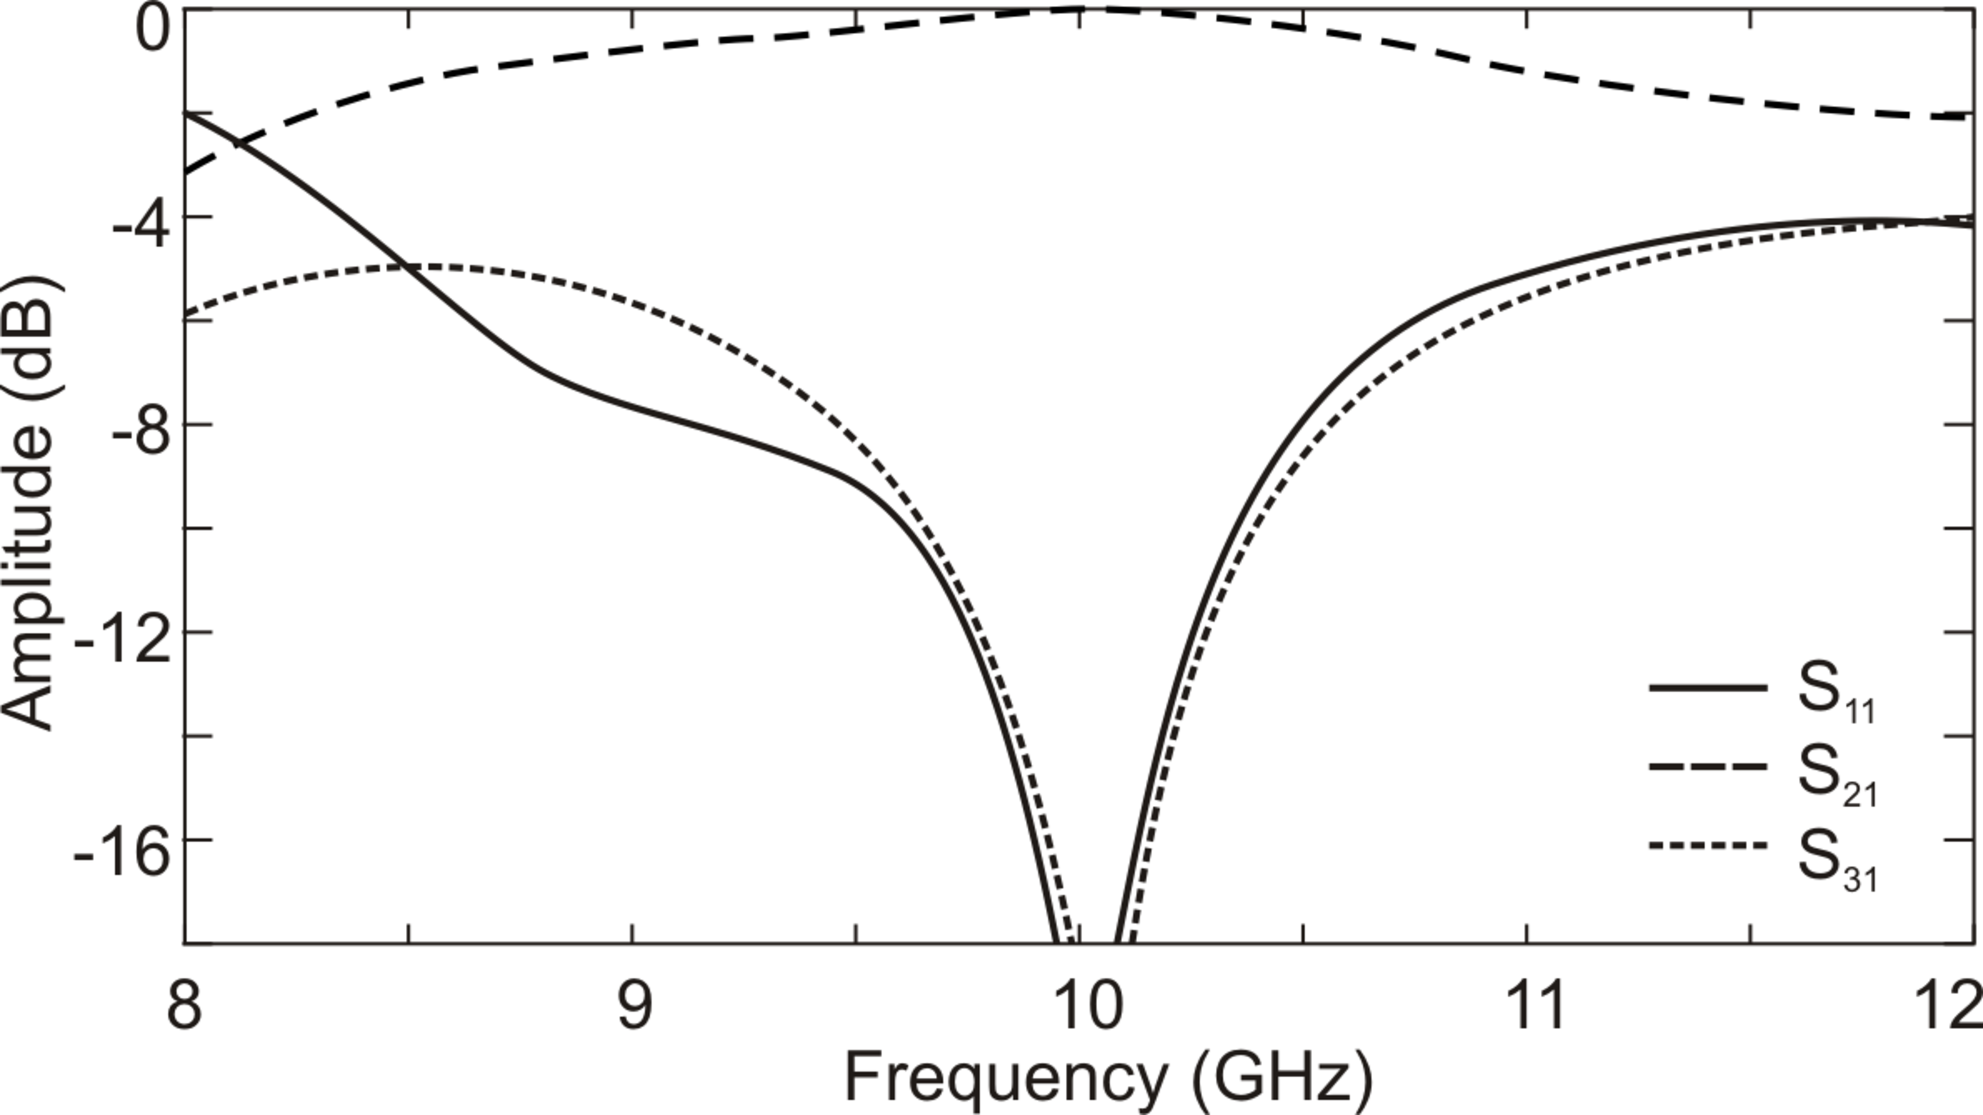
\includegraphics[width=10cm]{circresplin}
\caption{Circulator's small signal frequency response.}
\label{fig:circresplin}
\end{figure}

\begin{figure}[!ht]
\centering
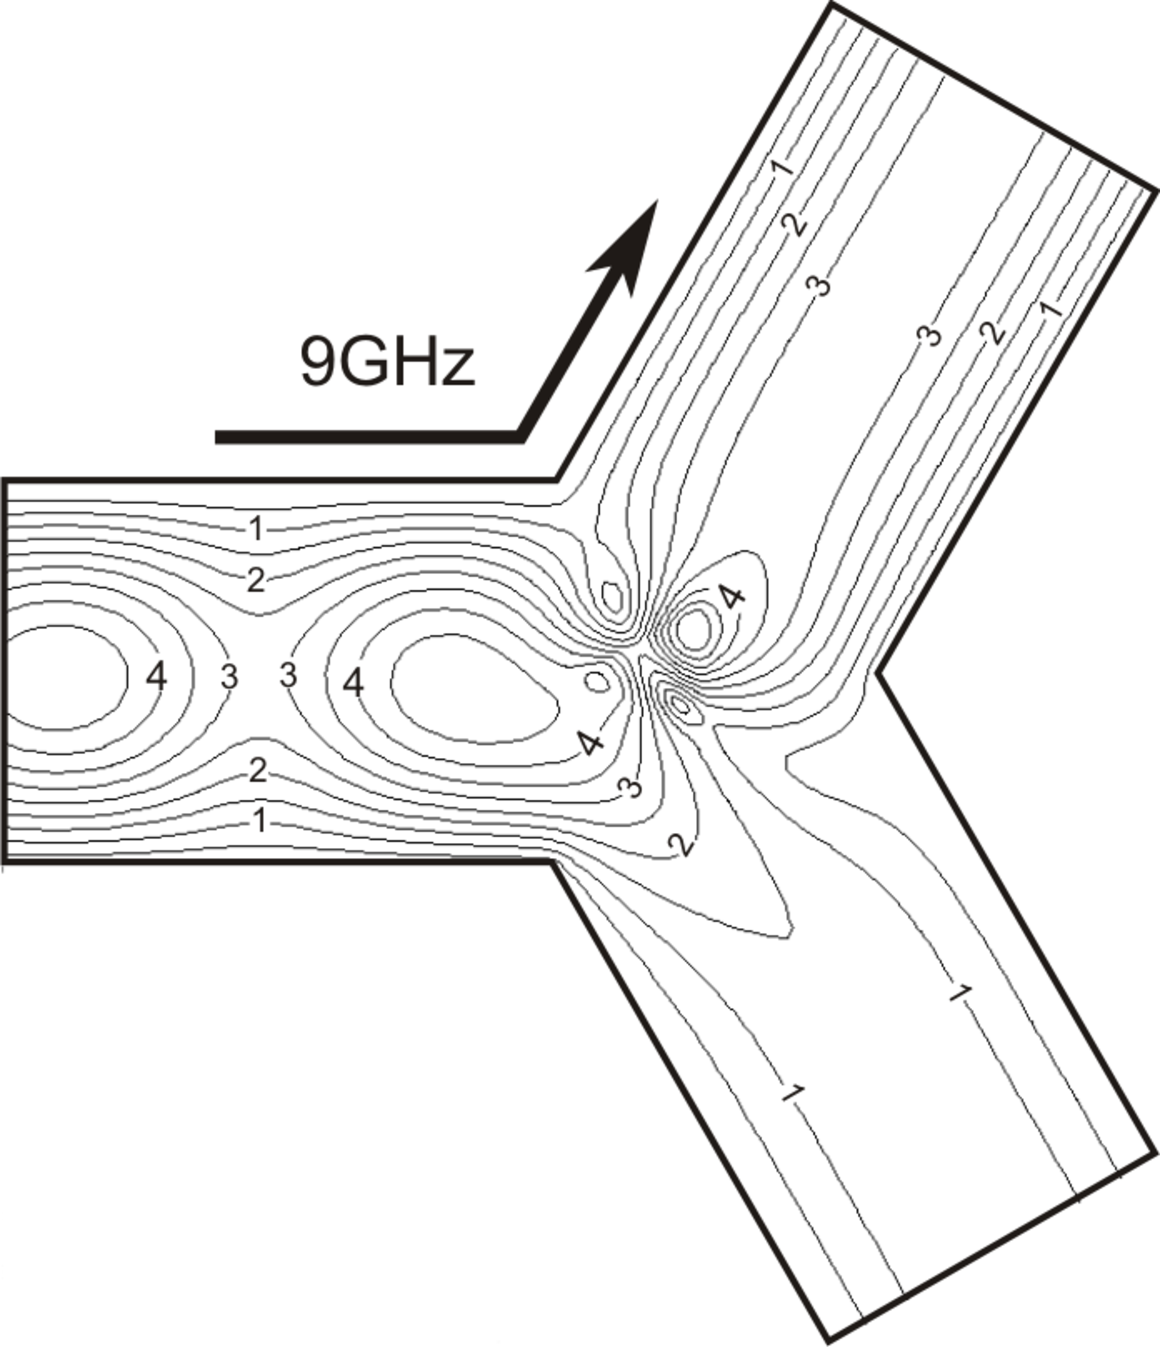
\includegraphics[width=8cm]{linfield}
\caption{Electric field $\left(\frac{\mathrm{kV}}{\mathrm{m}}\right)$ distribution at 9~GHz for 1~W impinging on $\Gamma_1$.}
\label{fig:linfield}
\end{figure}
 
To assess the nonlinearity of the modeled device, the circulator is analyzed assuming a strong interfering signal impinging on the isolated port ($\Gamma_3$) at $f_i = 10~\mathrm{GHz}$, 10 dB higher than the signal at Port 1, being the signal frequency $f_s \in [8,12]~\mathrm{GHz}$, engendering undesired intermodulation products (IMPs) at the coupled port ($\Gamma_2$). The convergence of the harmonic orders ($P$) is analyzed upon increasing the order progressively and monitoring the power kept by in-band IMPs signals ($2f_i-f_s$ and $2f_s-f_i$). The order of $G$ is chosen such that  $G\omega_g = \max(\omega_{\{p\}})$, $\omega_g = \gcd(\omega_i,\omega_s)$. For this test, the signal power impinging at $f_s = 9$~GHz has been assumed of 150~W, and the interferer one of 1.5~kW at $f_i = 10$~GHz. An iteration loop stop criterion $\tau = 10^{-9}$ has been assumed. Results are shown in table \ref{tab:power}, while Fig. \ref{fig:nlfield} reports the fieldmaps at the signal and interferent frequencies, as well as the in-band interferent. 
%
\begin{sidewaystable}[h]
\begin{center}
\begin{tabular}{|c|c|c|c|c|}
\hline 
& \multicolumn{4}{c|}{Harmonic order considered (cumulative from left to right)} \\ \hline
\multirow{2}{*}{Harmonic order} & \multirow{2}{*}{ Only $2f_1-f_2$, $2f_2-f_1$} & $2f_1+f_2$, $2f_2+f_1$, &	$f_1+f_2$, $|f_1-f_2|$, & $3f_1-2f_2$, $3f_2-2f_1$,\\
& & $3f_1$, $3f_2$ (all $3^\mathrm{rd}$ order) & $2f_1$, $2f_2$ (all $2^\mathrm{nd}$ order) &  $3f_1+2f_2$, $3f_2+2f_1$\\ \hline \hline
Power at $2f_1-f_2$~[W]& $4.6019~10^{-3}$ & $4.2246~10^{-3}$ & $4.2246~10^{-3}$ & $4.2186~10^{-3}$\\ \hline
Power at $2f_2-f_1$~[W]& $2.0990~10^{-1}$ & $2.1951~10^{-1}$ & $2.1951~10^{-1}$ & $2.1991~10^{-1}$\\ \hline
\end{tabular}
\end{center}
\caption{Harmonic power at third order intermodulation products as $P$ is increased.}
\label{tab:power}
\end{sidewaystable} 
%
\clearpage

\begin{figure}[!ht]
\centering
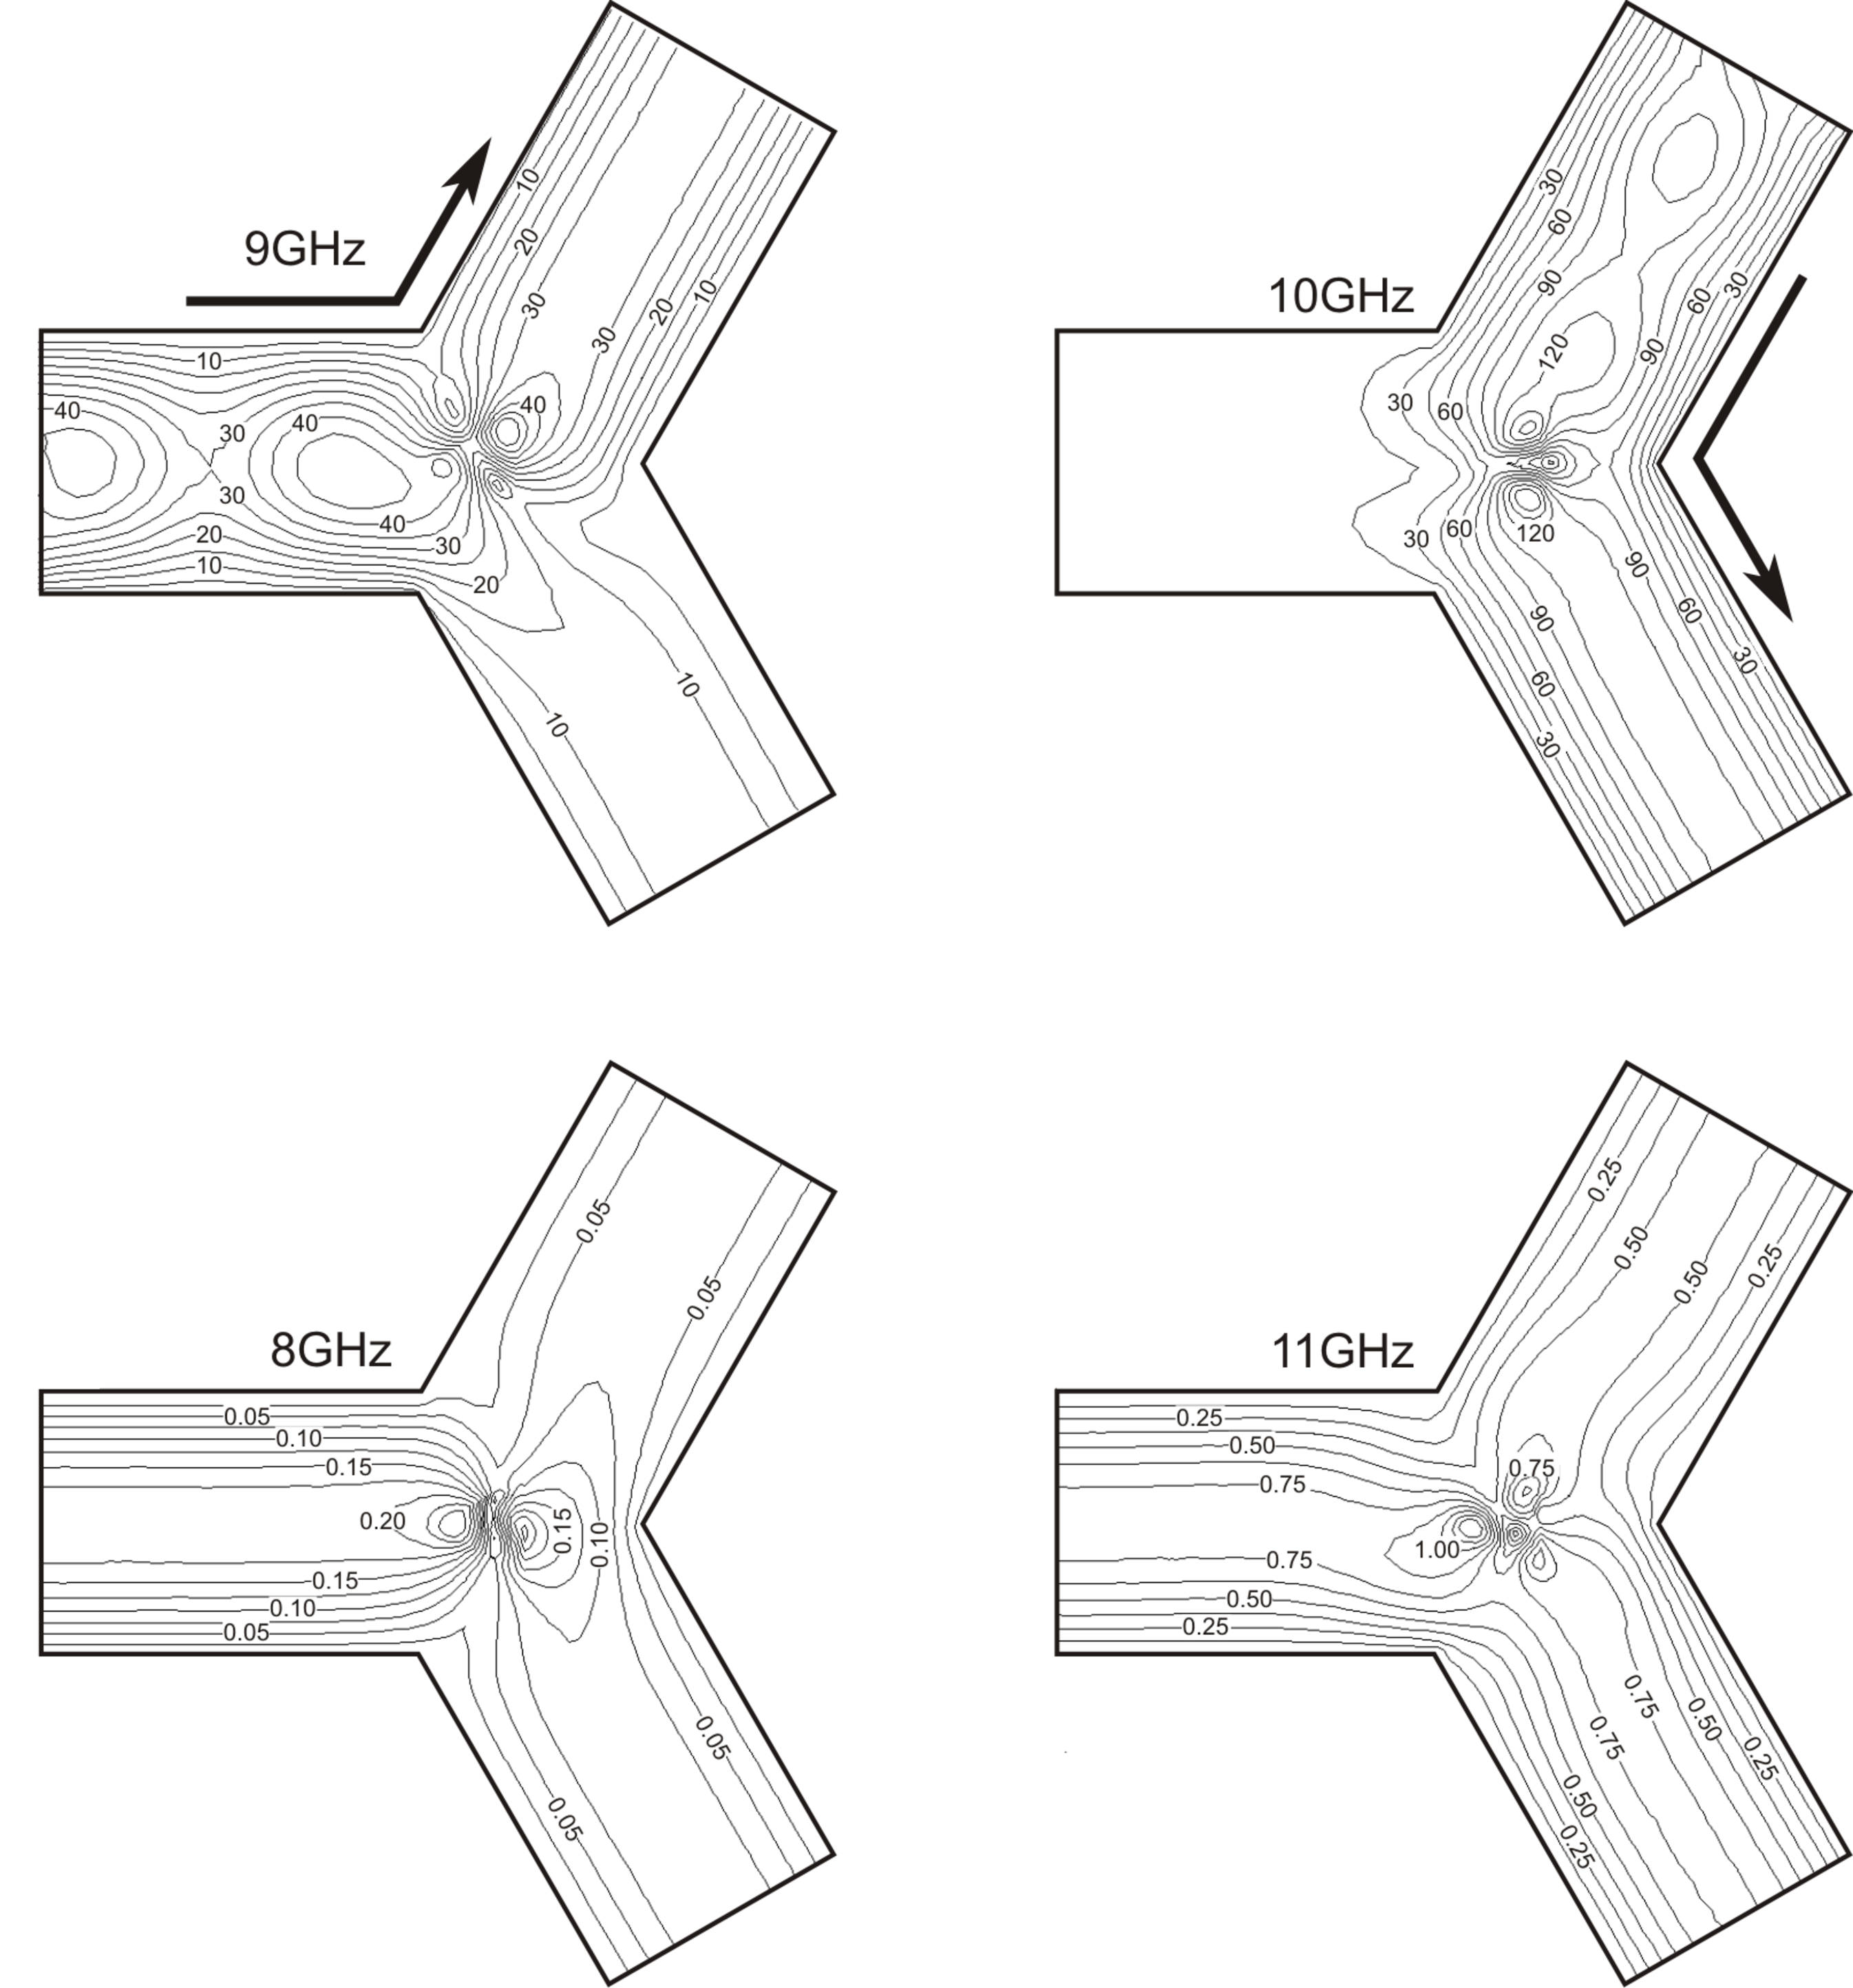
\includegraphics[width=13.4cm]{nlfield}
\caption{Electric field $\left(\frac{\mathrm{kV}}{\mathrm{m}}\right)$ distribution for the third order intermodulation problem, at 9 GHz, 10 GHz, and at in-band IMPs frequencies 8 and 11 GHz.}
\label{fig:nlfield}
\end{figure}

It is worth noticing that as the harmonic order grows, higher order TE modes at ports boundaries become propagating, and hence 10 modes \cite{pelosi2009quick} have been retained to accurately compute the power balance.


Even if the exact (continuous) solution cannot be achieved, table \ref{tab:power} shows that the computation of in-band third order products, considering up to all the third order products, leads to a maximum error of less than 0.2~\%. In this case, Figs. \ref{fig:f1} and \ref{fig:f2} shows the resulting power amplitudes as a function of frequency for the two in-band third-order IMPs for different signal and interferent power levels. The power delivered to IMPs is in good agreement with those reported in \cite{how1997nonlinear}.

\begin{figure}[!ht]
\centering
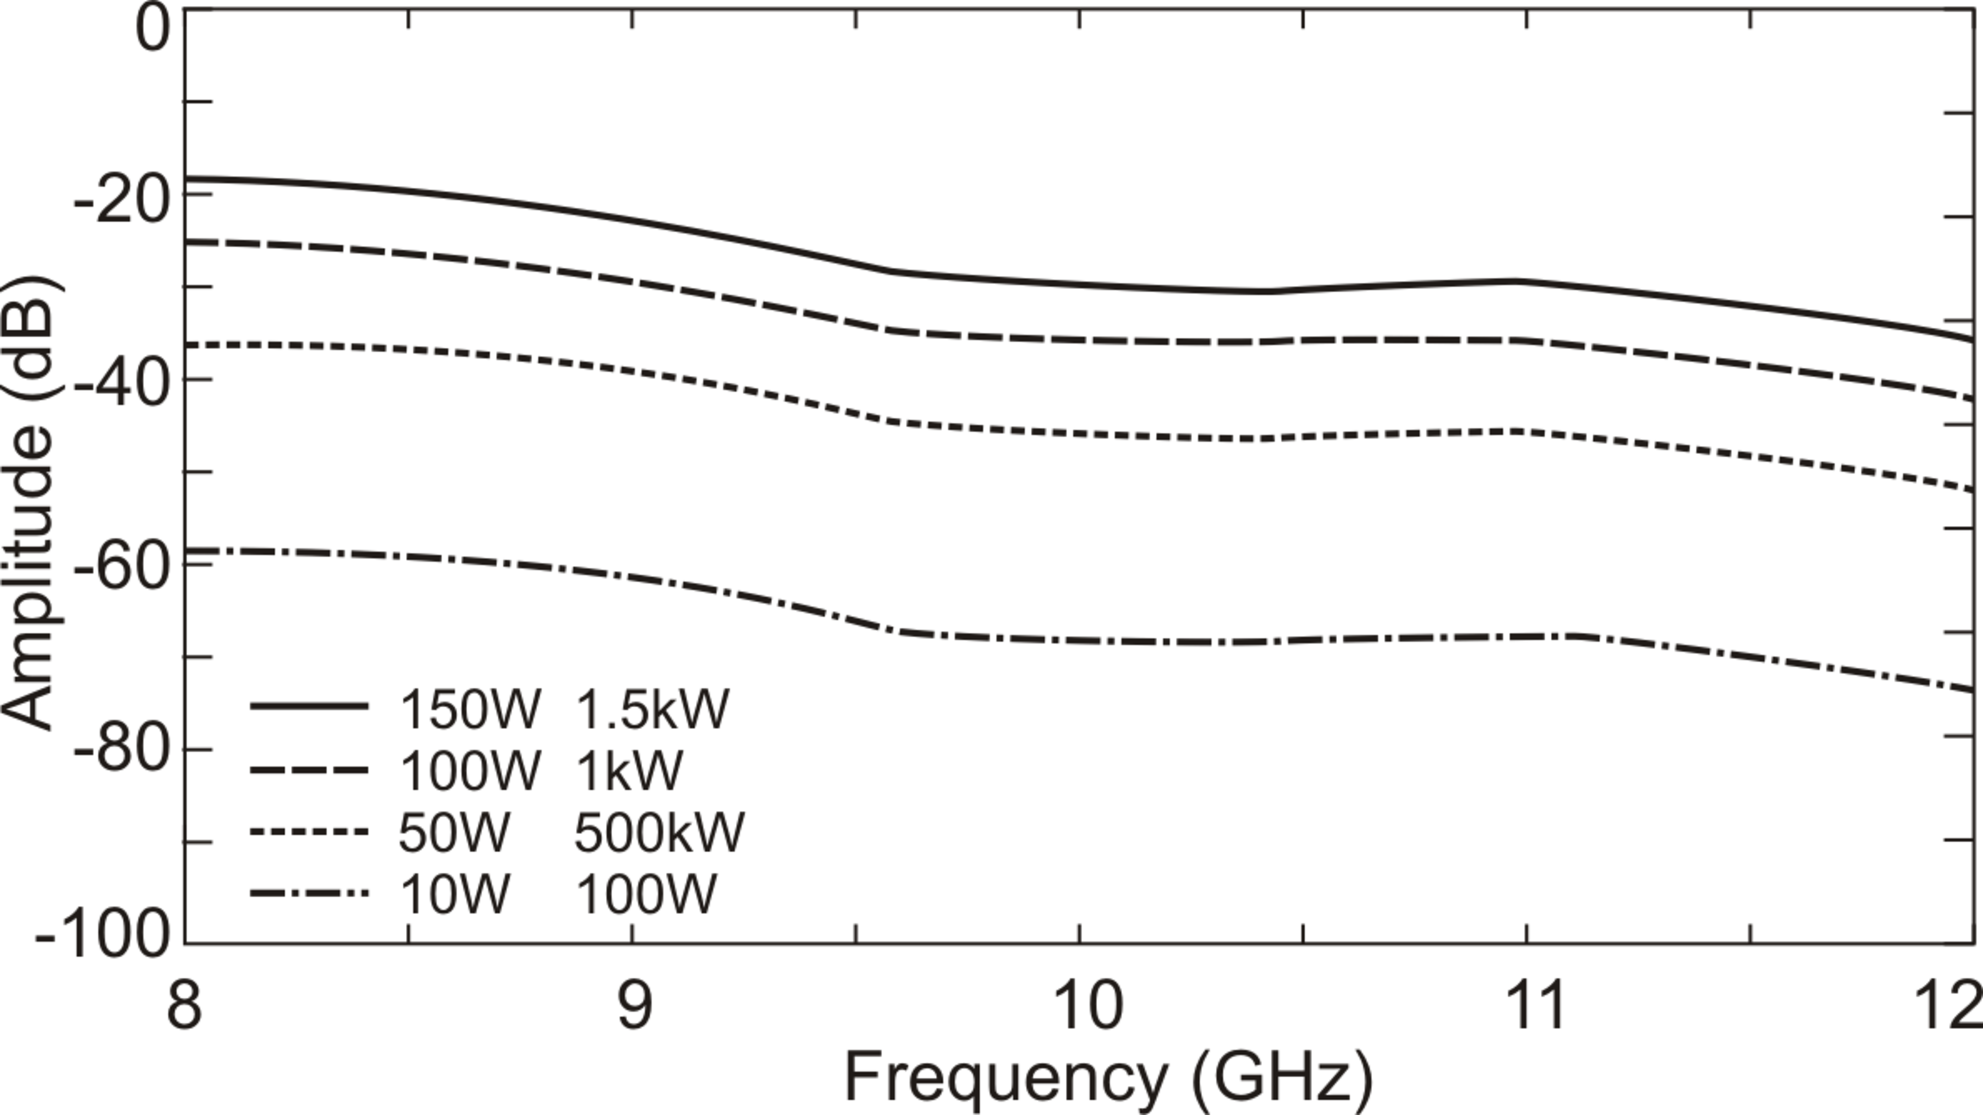
\includegraphics[width=10cm]{f1}
\caption{Intermodulation product power at $2 f_s - f_i$ ($f_i$~=~10~GHz).}
\label{fig:f1}
\end{figure}

\begin{figure}[!ht]
\centering
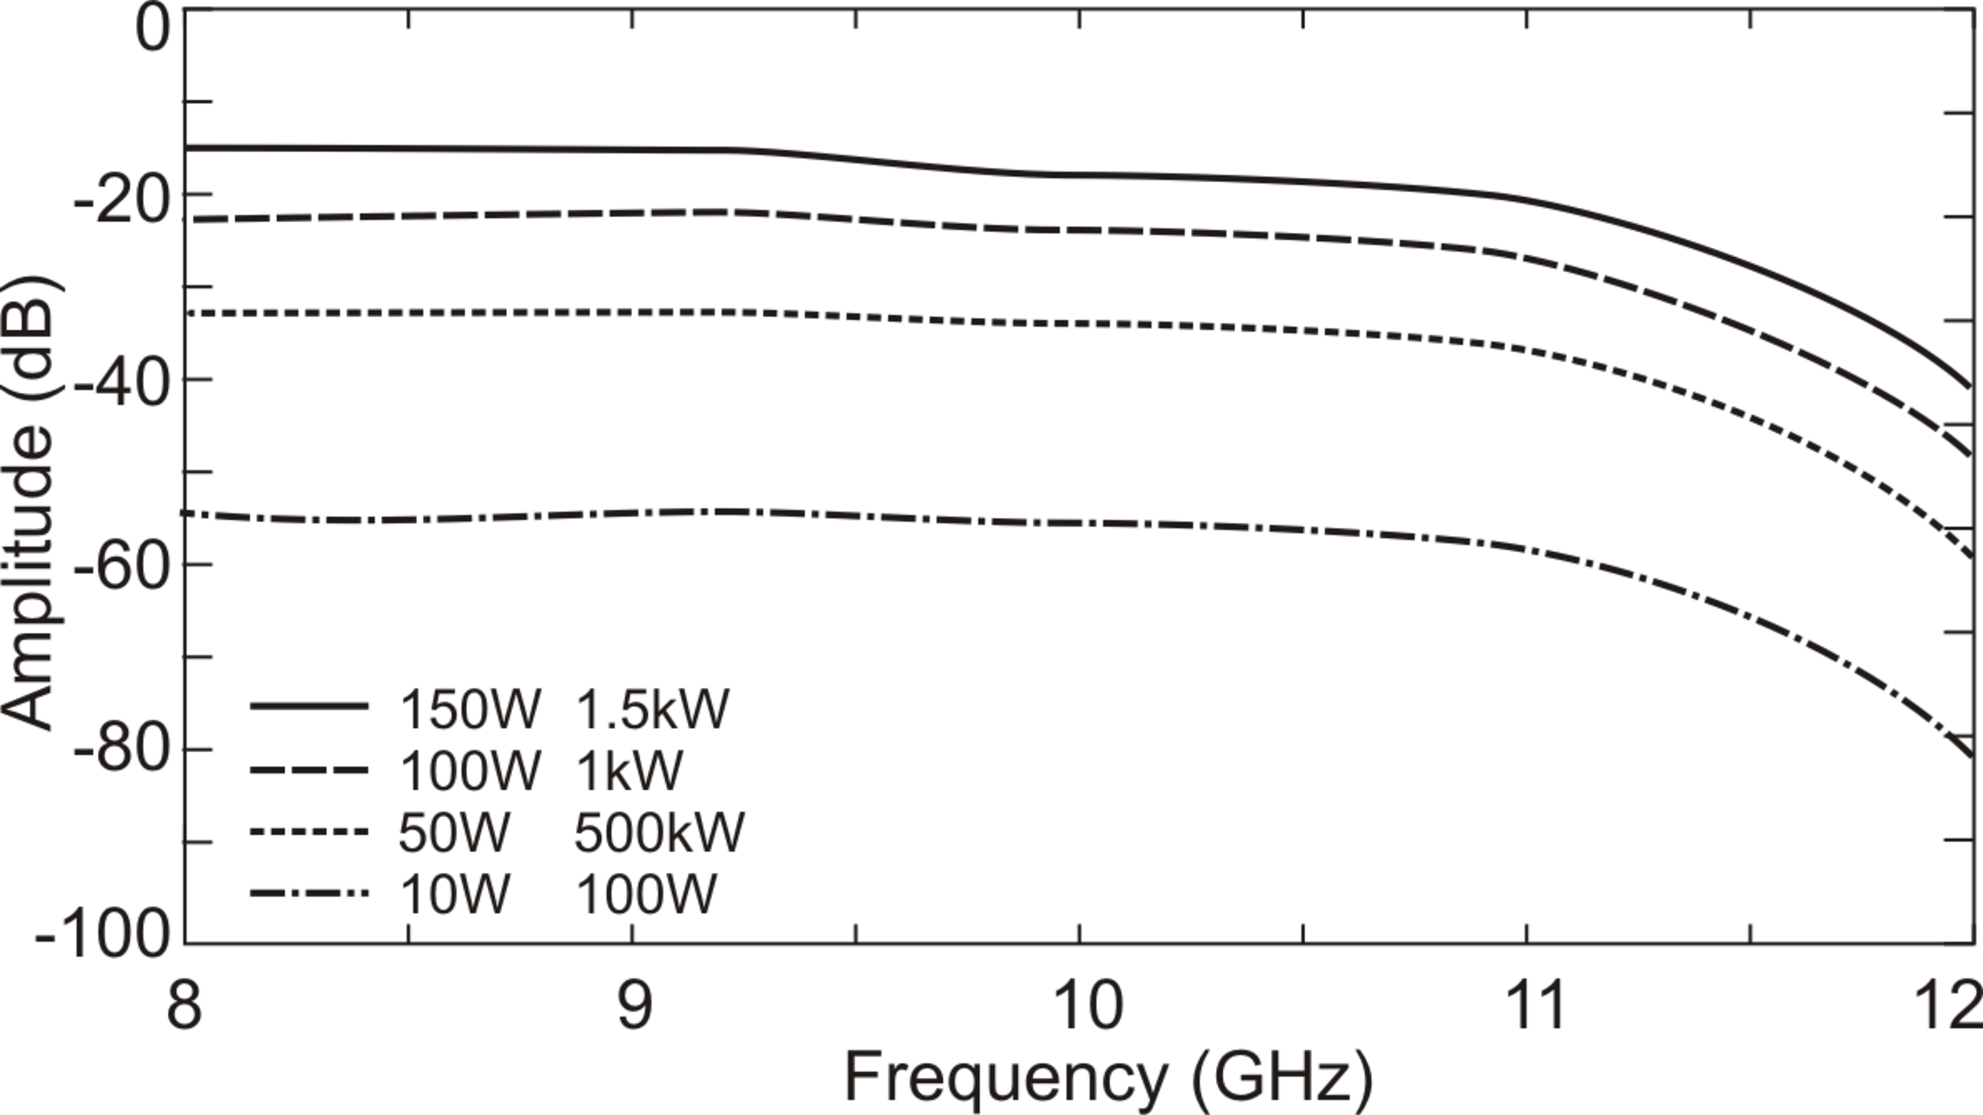
\includegraphics[width=10cm]{f2}
\caption{Intermodulation product power at $2 f_i - f_s$ ($f_i$~=~10~GHz).}
\label{fig:f2}
\end{figure}

Also here a Schur based domain decomposition (DD) scheme, which provides the same solution of the standard full system iteration scheme, allows to speed up the computations. The acceleration of the DD solver, defined as the ratio between the standard scheme times (assembly and solve for whole domain at each iteration) and the DD times (assembly and solve for whole domain only at first iteration, then assembly and solve for nonlinear subdomains only), is reported in Fig. \ref{fig:accelerationorder}. Sparse direct solvers of a Matlab${}^\text{\circledR}$ implementation for both standard full and DD schemes have been employed to perform the computations.
%
\begin{figure}[!ht]
\centering
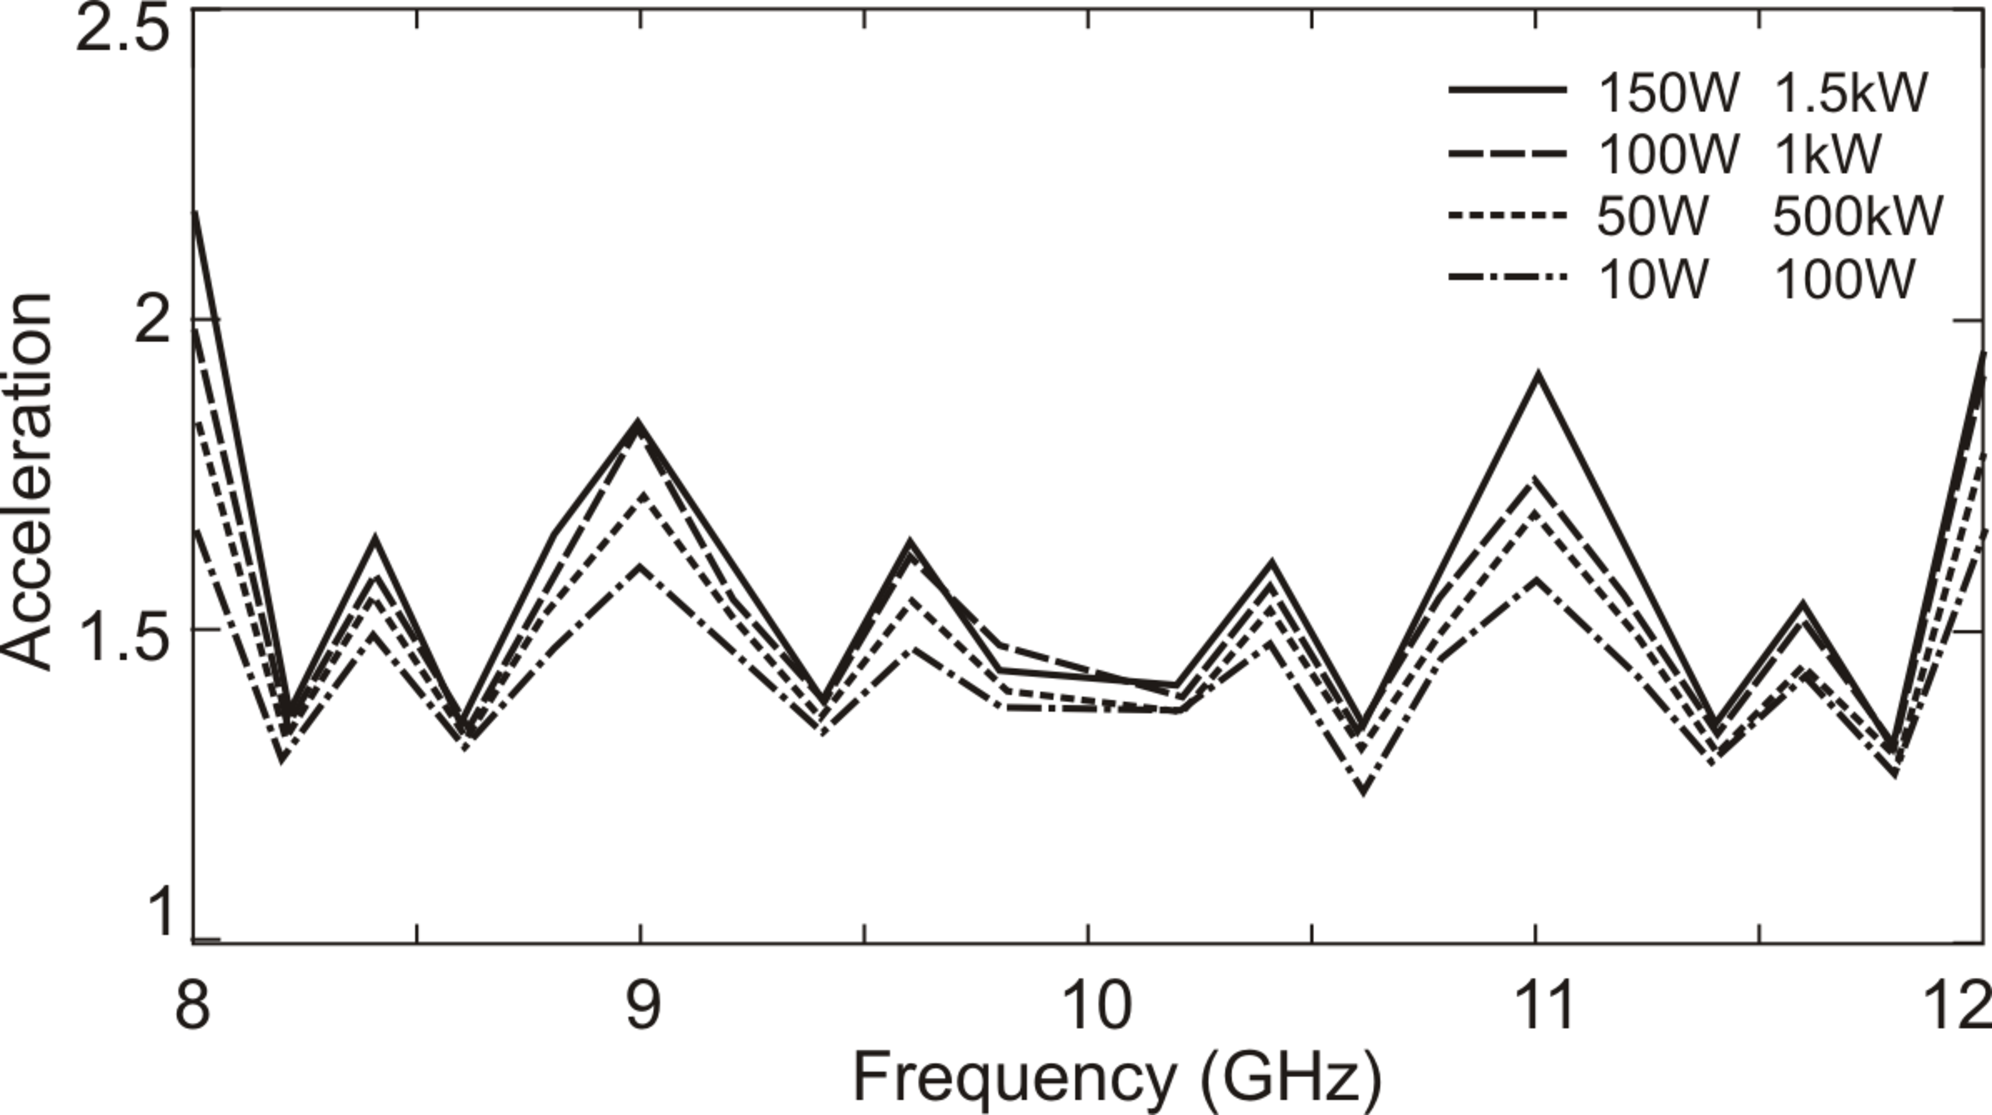
\includegraphics[width=10cm]{acccirc}
\caption{Acceleration of the DD scheme vs conventional scheme. Linear elements have been considered,
leading to 700 degrees of freedom and 8100 non-zero entries of [A].}
\label{fig:acccirc}
\end{figure}
%
All over the frequency sweep, the FFT-based algorithm employed to compute nonlinear materials testing has
required noticeably different amount of times, bound to differences in the number of iterations required,
leading to different values of acceleration for the chosen frequency points. The time step required to
accurately compute the testing integrals strongly depend on the difference between signal and interferer
frequencies. However, 45~\% to 60~\% average speed-up have been noticed within the signal bandwidth.

Further tests are performed to assess the efficiency of the method, both for 2 and 5 subdomains (only 1 with
nonlinear ferrite), while increasing the number of degrees of freedom (hence the non-zero entries of the
system matrix $\mat{A}$) by increasing the elements order from first to fourth (Fig. \ref{fig:acccirc} and \ref{fig:memcirc}).

\begin{figure}[!ht]
\centering
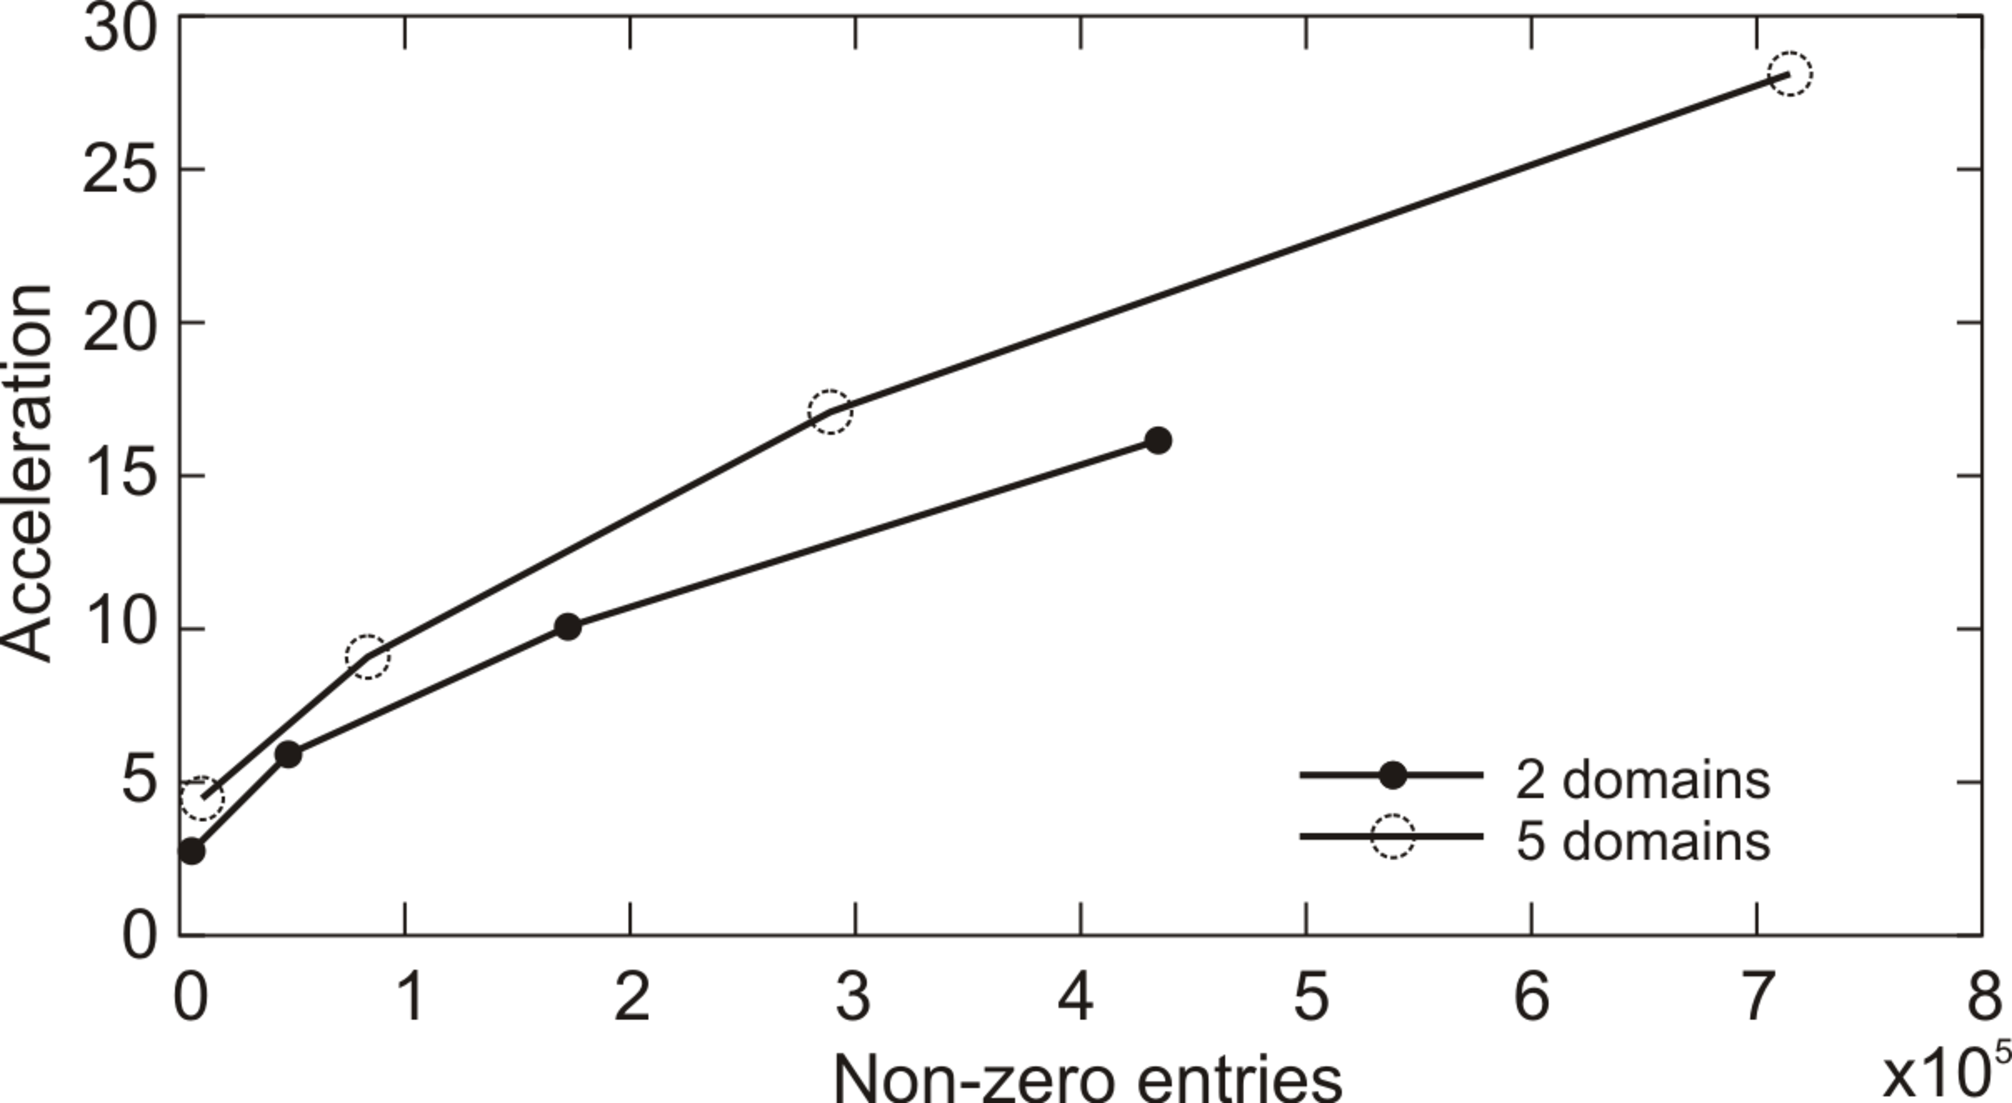
\includegraphics[width=10cm]{accelerationorder}
\caption{Acceleration of the DD scheme vs standard full scheme as a function of non-zero entries of $\mat{A}$.}
\label{fig:accelerationorder}
\end{figure}

The higher is the number of linear subdomains, the smaller are the submatrices of the linear subdomains,
leading to improved acceleration. Furthermore, acceleration grows logarithmically with the polynomial
order, that is with the number of non-zero entries of the system matrix.

\begin{figure}[!ht]
\centering
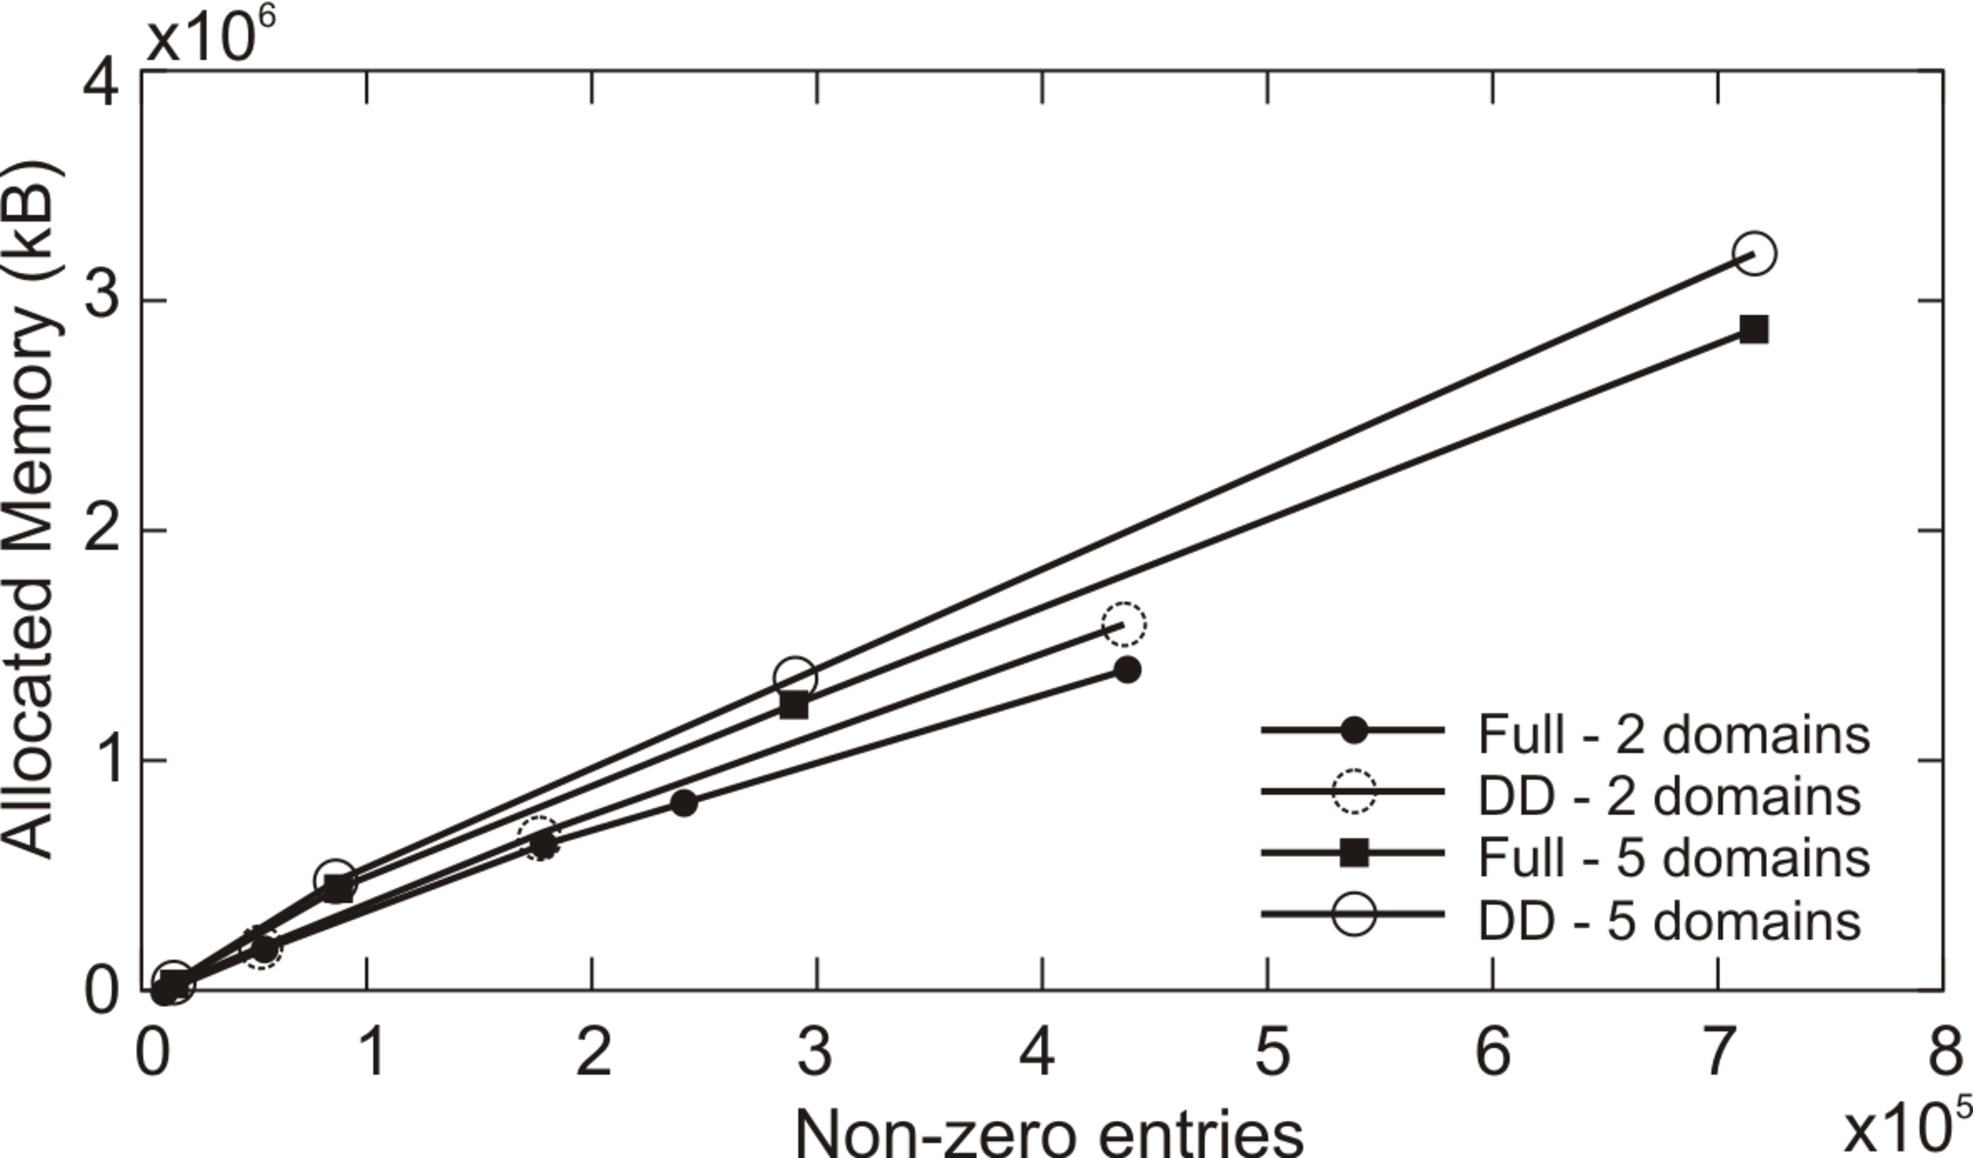
\includegraphics[width=10cm]{memcirc}
\caption{Allocated memory (stored and dynamically freed) as a function of non-zero entries of $\mat{A}$.}
\label{fig:memcirc}
\end{figure}

Increasing the number of subdomains generally leads to higher allocated memory. This is mainly due to an
increase of geometrical and finite elements unknowns reordering information, which is kept in both standard
full and DD schemes. DD schemes require more memory to store the Schur complement matrices and solve
for related unknowns.


\subsection{Barium strontium titanate thin film coplanar waveguide}

The present test represent a first attempt to analyze the validity of the HBFE method to a 3D structure whose high-order harmonics measurements have been reported in \cite{mateu2006measurements}. 

\begin{figure}[ht!]
\centering
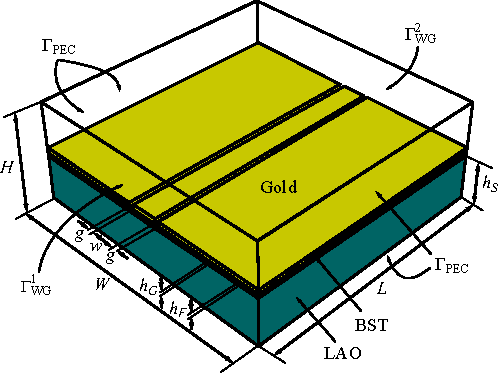
\includegraphics[width=10cm]{CPW}
\caption{Sketch of the coplanar waveguide as the domain $\Omega$ of HBFE analysis and relative boundaries $\Gamma_\text{PEC}$ for the perfect electric conductor shield and waveports boundary conditions on $\Gamma_\text{WG}^1$ and $\Gamma_\text{WG}^2$. The center conductor of the strip is $w = 20~{\mu}$m with $g = 20~{\mu}$m gaps on both sides and $h_G = 0.3~{\mu}$m of thickness. The thickness of the BST thin-film is $h_F = 400$~nm-thick and that of the LAO substrate is $h_S = 500~{\mu}$m. Dimensions of the box are $W=2$~mm, $H=1$~mm and $L=0.42$~mm.}
\label{fig:CPW}
\end{figure}

It consists of a coplanar waveguide (CPW) transmission line as depicted in Fig. \ref{fig:CPW}. A $400$~nm $\text{Ba}_{0.3}\text{Sr}_{0.7}\text{TiO}_{3}$ (BST) thin film grown on a $\text{LaAlO}_3$ (LAO) substrate. \cite{mateu2006measurements} does not report the employed LAO substrate thickness, hence a typical value of $0.5~{\mu}$m \cite{gim2000microstructure} have been used. The gold conductors that constitutes the CPW are $0.3~{\mu}$m-thick. The center conductor linewidth is of $20~{\mu}$m and so are the gaps around. The width (2~mm) and height (1~mm) of the shielding box walls are chosen far enough from the line such that the impedance of the dominant TEM mode slightly depend on the perfect electric walls, the dominant coplanar mode field being concentrated within the gaps. Furthermore, the mesh of the structure is such that the coupling between the coplanar mode and other modes such as the stripline mode and higher-order hibrid TE and TM modes is minimized within the frequency range of analysis. 
Material properties for the linear case are set as reported in table \ref{tab:CPWmat}, where $\bar{\epsilon}'$ and $\bar{\epsilon}''$ are, respectively, the real and imaginary parts of the permittivity.

\begin{table}[h!]
\begin{center}
\begin{tabular}{|c|c|c|c|c|} \hline
Material & ${\bar{\epsilon}'}_r$ & $\bar{\mu}_r$ & $\bar{\sigma}~\mat{\frac{\mathrm{S}}{\mathrm{m}}}$ & $\tan \delta = \frac{\bar{\epsilon}''}{\bar{\epsilon}'}$ \\ \hline \hline
LAO & 24 & 1 & 0 & 0 \\ \hline
BST & 475 & 1 & 0 & 0.0842 \\ \hline
Gold & 1 & 0.99996 & $4.1~10^7$ & 0 \\ \hline
Vacuum & 1 & 1 & 0 & 0 \\ \hline
\end{tabular}
\end{center}
\caption{Material properties for the linear CPW.}
\label{tab:CPWmat}
\end{table} 

In the nonlinear case, the BST film has the following Kerr-like permittivity (real part)
\begin{equation}
\tilde{{\varepsilon}'}_r(\mathbf{E}, \mathbf{r}) = {\bar{\varepsilon}'}_r \left( 1 + 
\alpha_2 \ |\mathbf{E}|^2 \right), \qquad \mathbf{r} \in \Omega_2
\end{equation}
\noindent with $\alpha_2 = - 5.01~10^{-14}~\frac{\mathrm{m}^2}{\mathrm{V}^2}$ as derived from measurements in \cite{mateu2006measurements}. The imaginary part has been left independent from the field intensity.

A first, linear, analysis is conducted with first order curl-conforming basis functions to ensure proper simulations setups. The choice of the basis order is motivated by the high mesh density within BST and gold materials, principally imposed by the thickness of these layers. The mesh is composed of 98~216 tetrahedra, 37~119 in the LAO substrate, 23~007 in the BST film, 13~441 in the gold strips and the remaining 24~619 in the vacuum. Three modes (transfinite element method) have been retained in the analysis while feeding the CPW only with the coplanar mode. The assembly has led to 112~899 unknowns, which is relatively high if we think of the electrical size. As introduced in chapter \ref{chap:INT}, this is the case of electrically small geometries and high permittivities that causes a small problem to become large. The scattering parameters  over the frequency range $[2,10]$~GHz are reported in Fig. \ref{fig:Scattering}. In particular, these show that the overall crosstalk between modes is below -35~dB all over the range. Furthermore, the stripline mode of the structure should be propagating if feeded at those frequencies.
%

\begin{figure}[ht!]
\centering
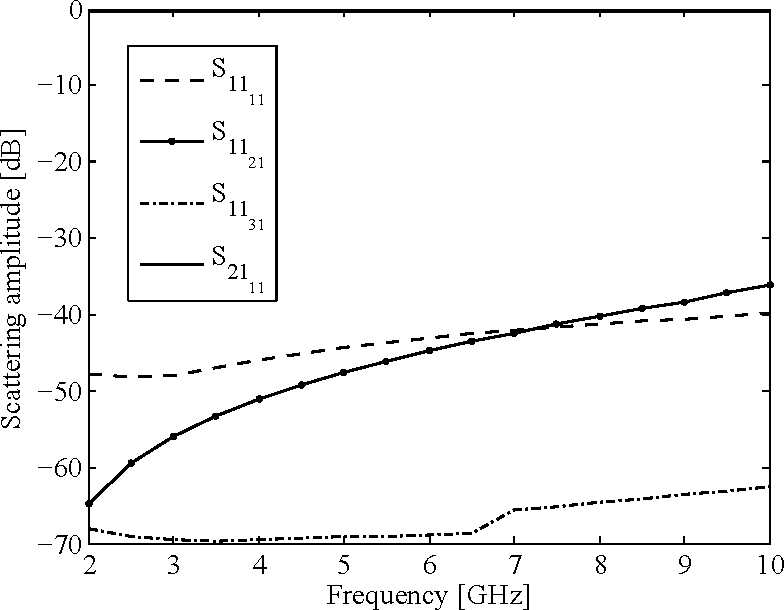
\includegraphics[width=10cm]{CPWlinScat}
\caption{Spectral response of the CPW ($S_{{\text{port1|port2}}_{\text{mode1|mode2}}}$). }
\label{fig:Scattering}
\end{figure}
%

Figs. \ref{fig:CPWlin1}, \ref{fig:CPWlin2} and \ref{fig:CPWlin3} show, respectively, the electric field when the coplanar, stripline and first hibrid TE mode are feeding the CPW at 6~GHz. The fields distributions clearly show that they are propagating, however, orthogonality between modes is such that the crosstalk remains below -35~dB.

\begin{figure}[h!]
\centering
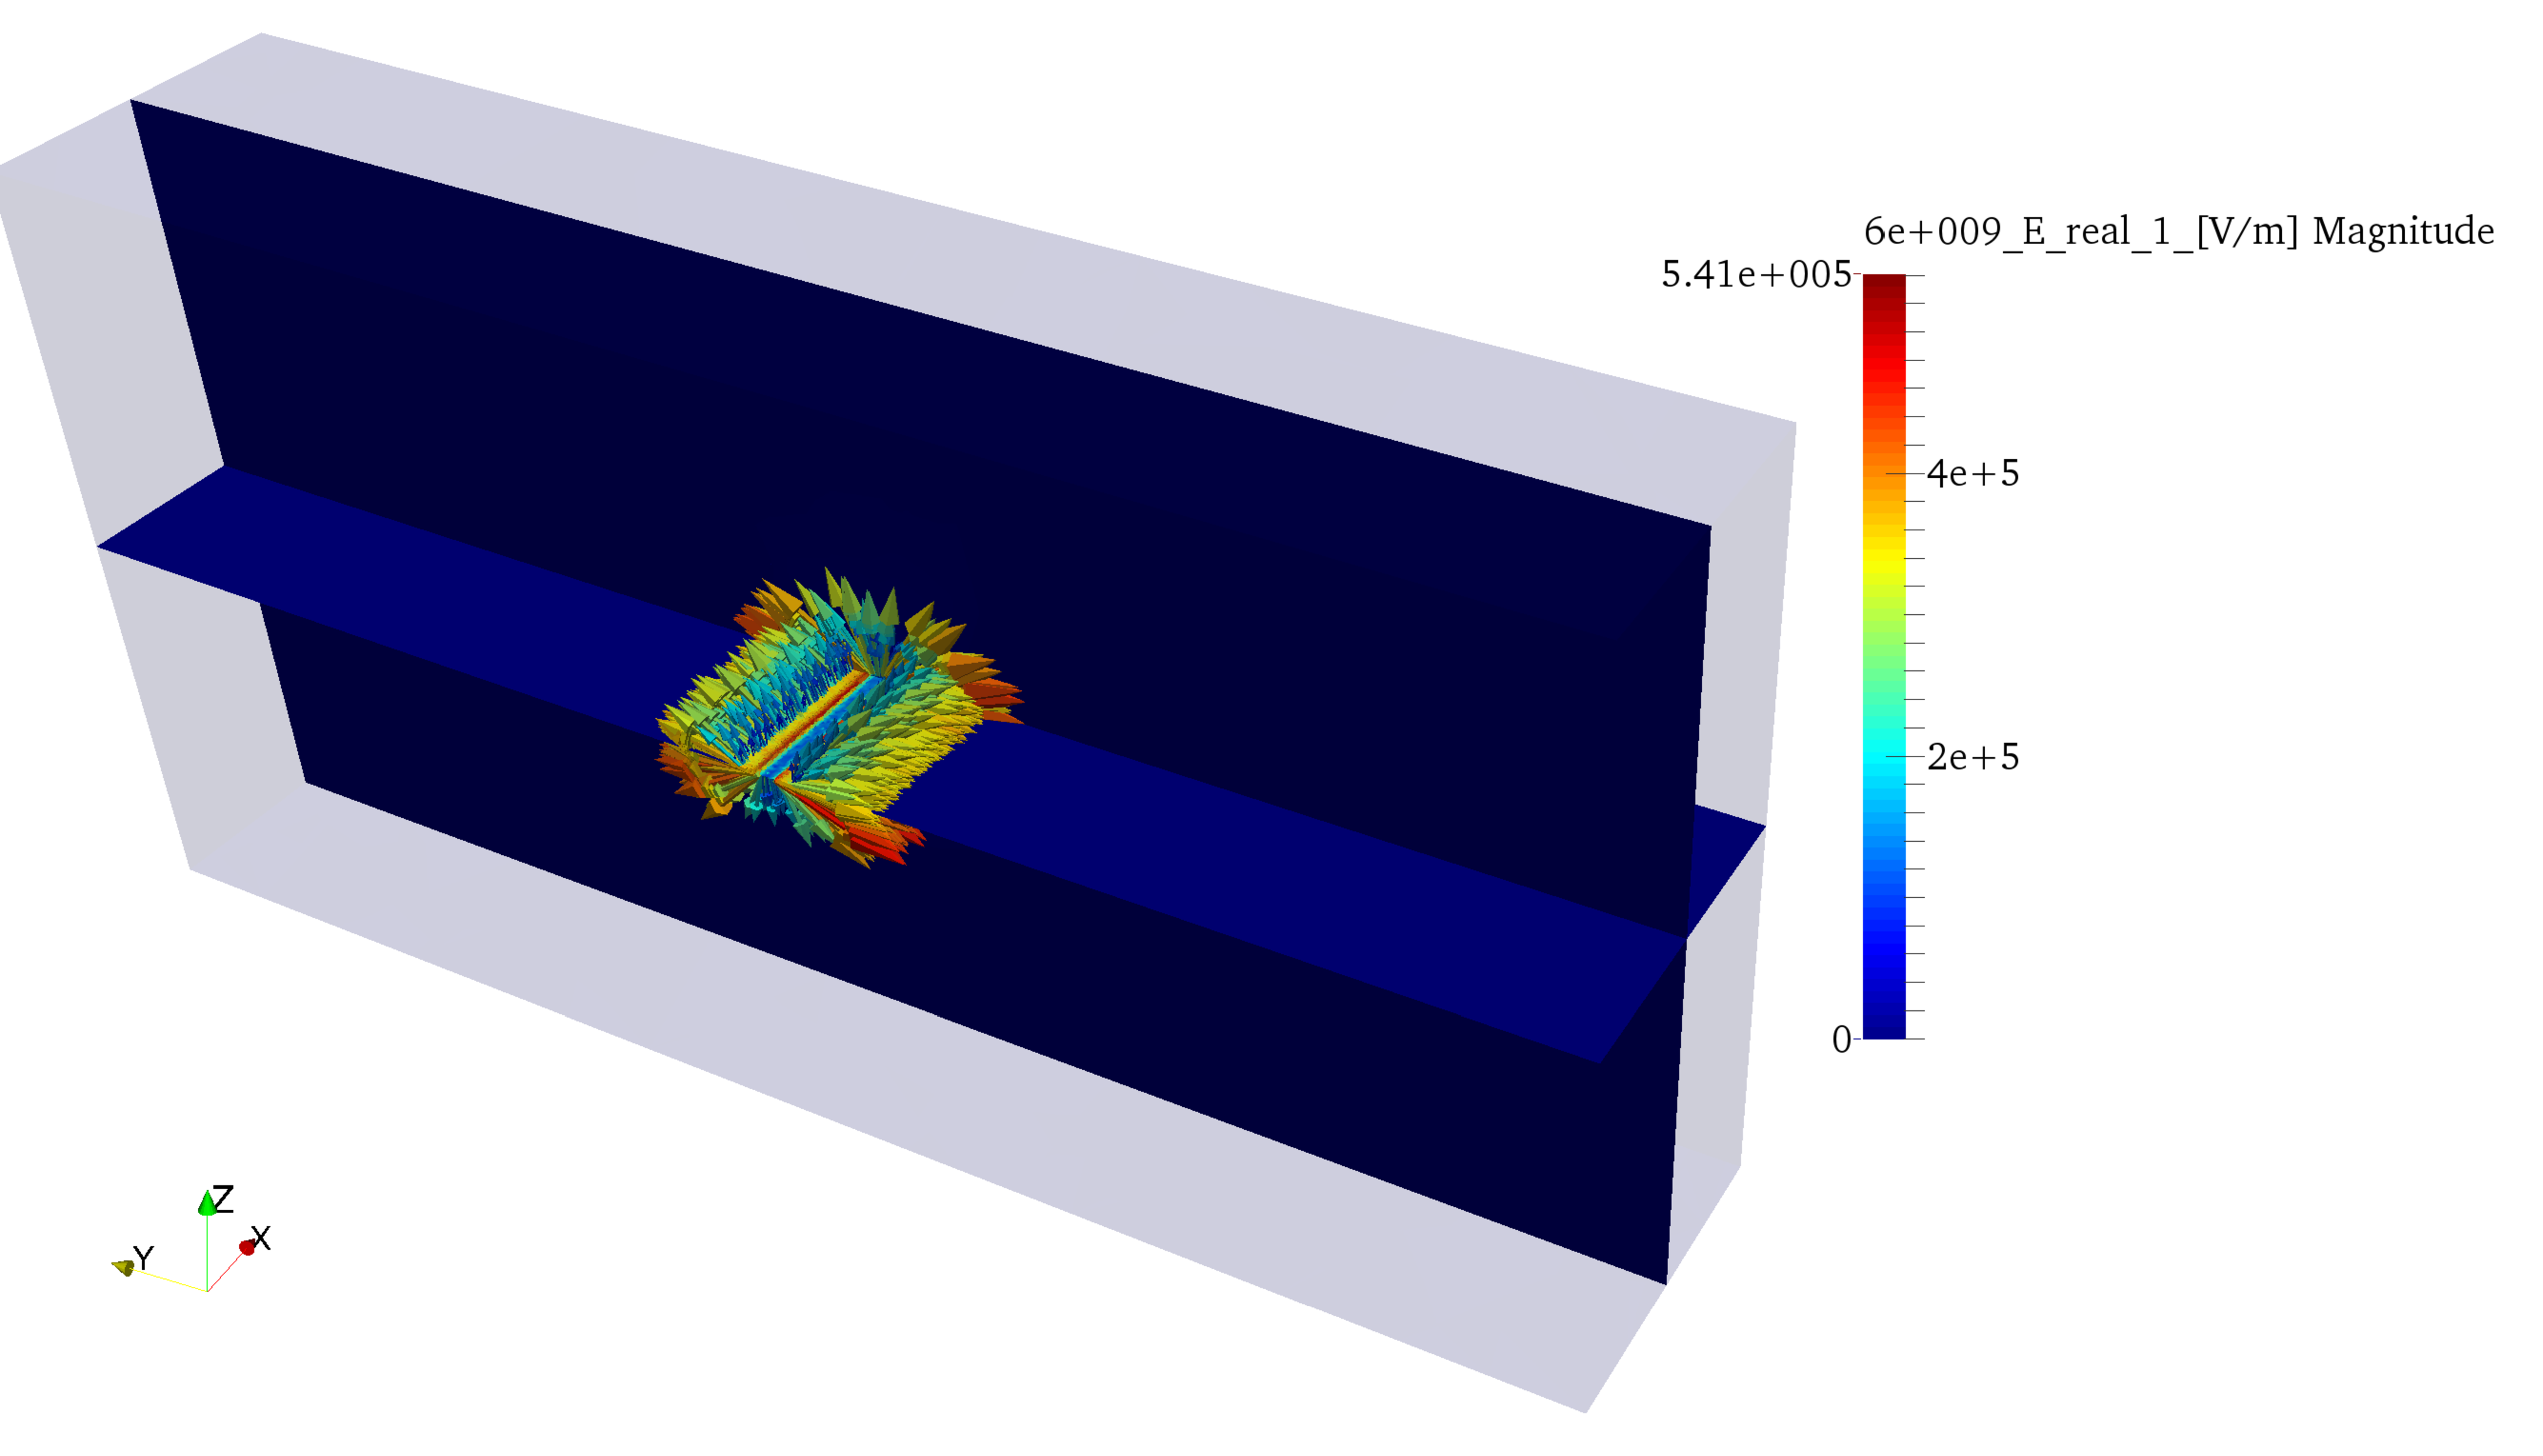
\includegraphics[width=13.4cm]{CPWlin1}
\caption{Coplanar mode traveling through the CPW at 6~GHz.}
\label{fig:CPWlin1}
\end{figure}
\begin{figure}[h!]
\centering
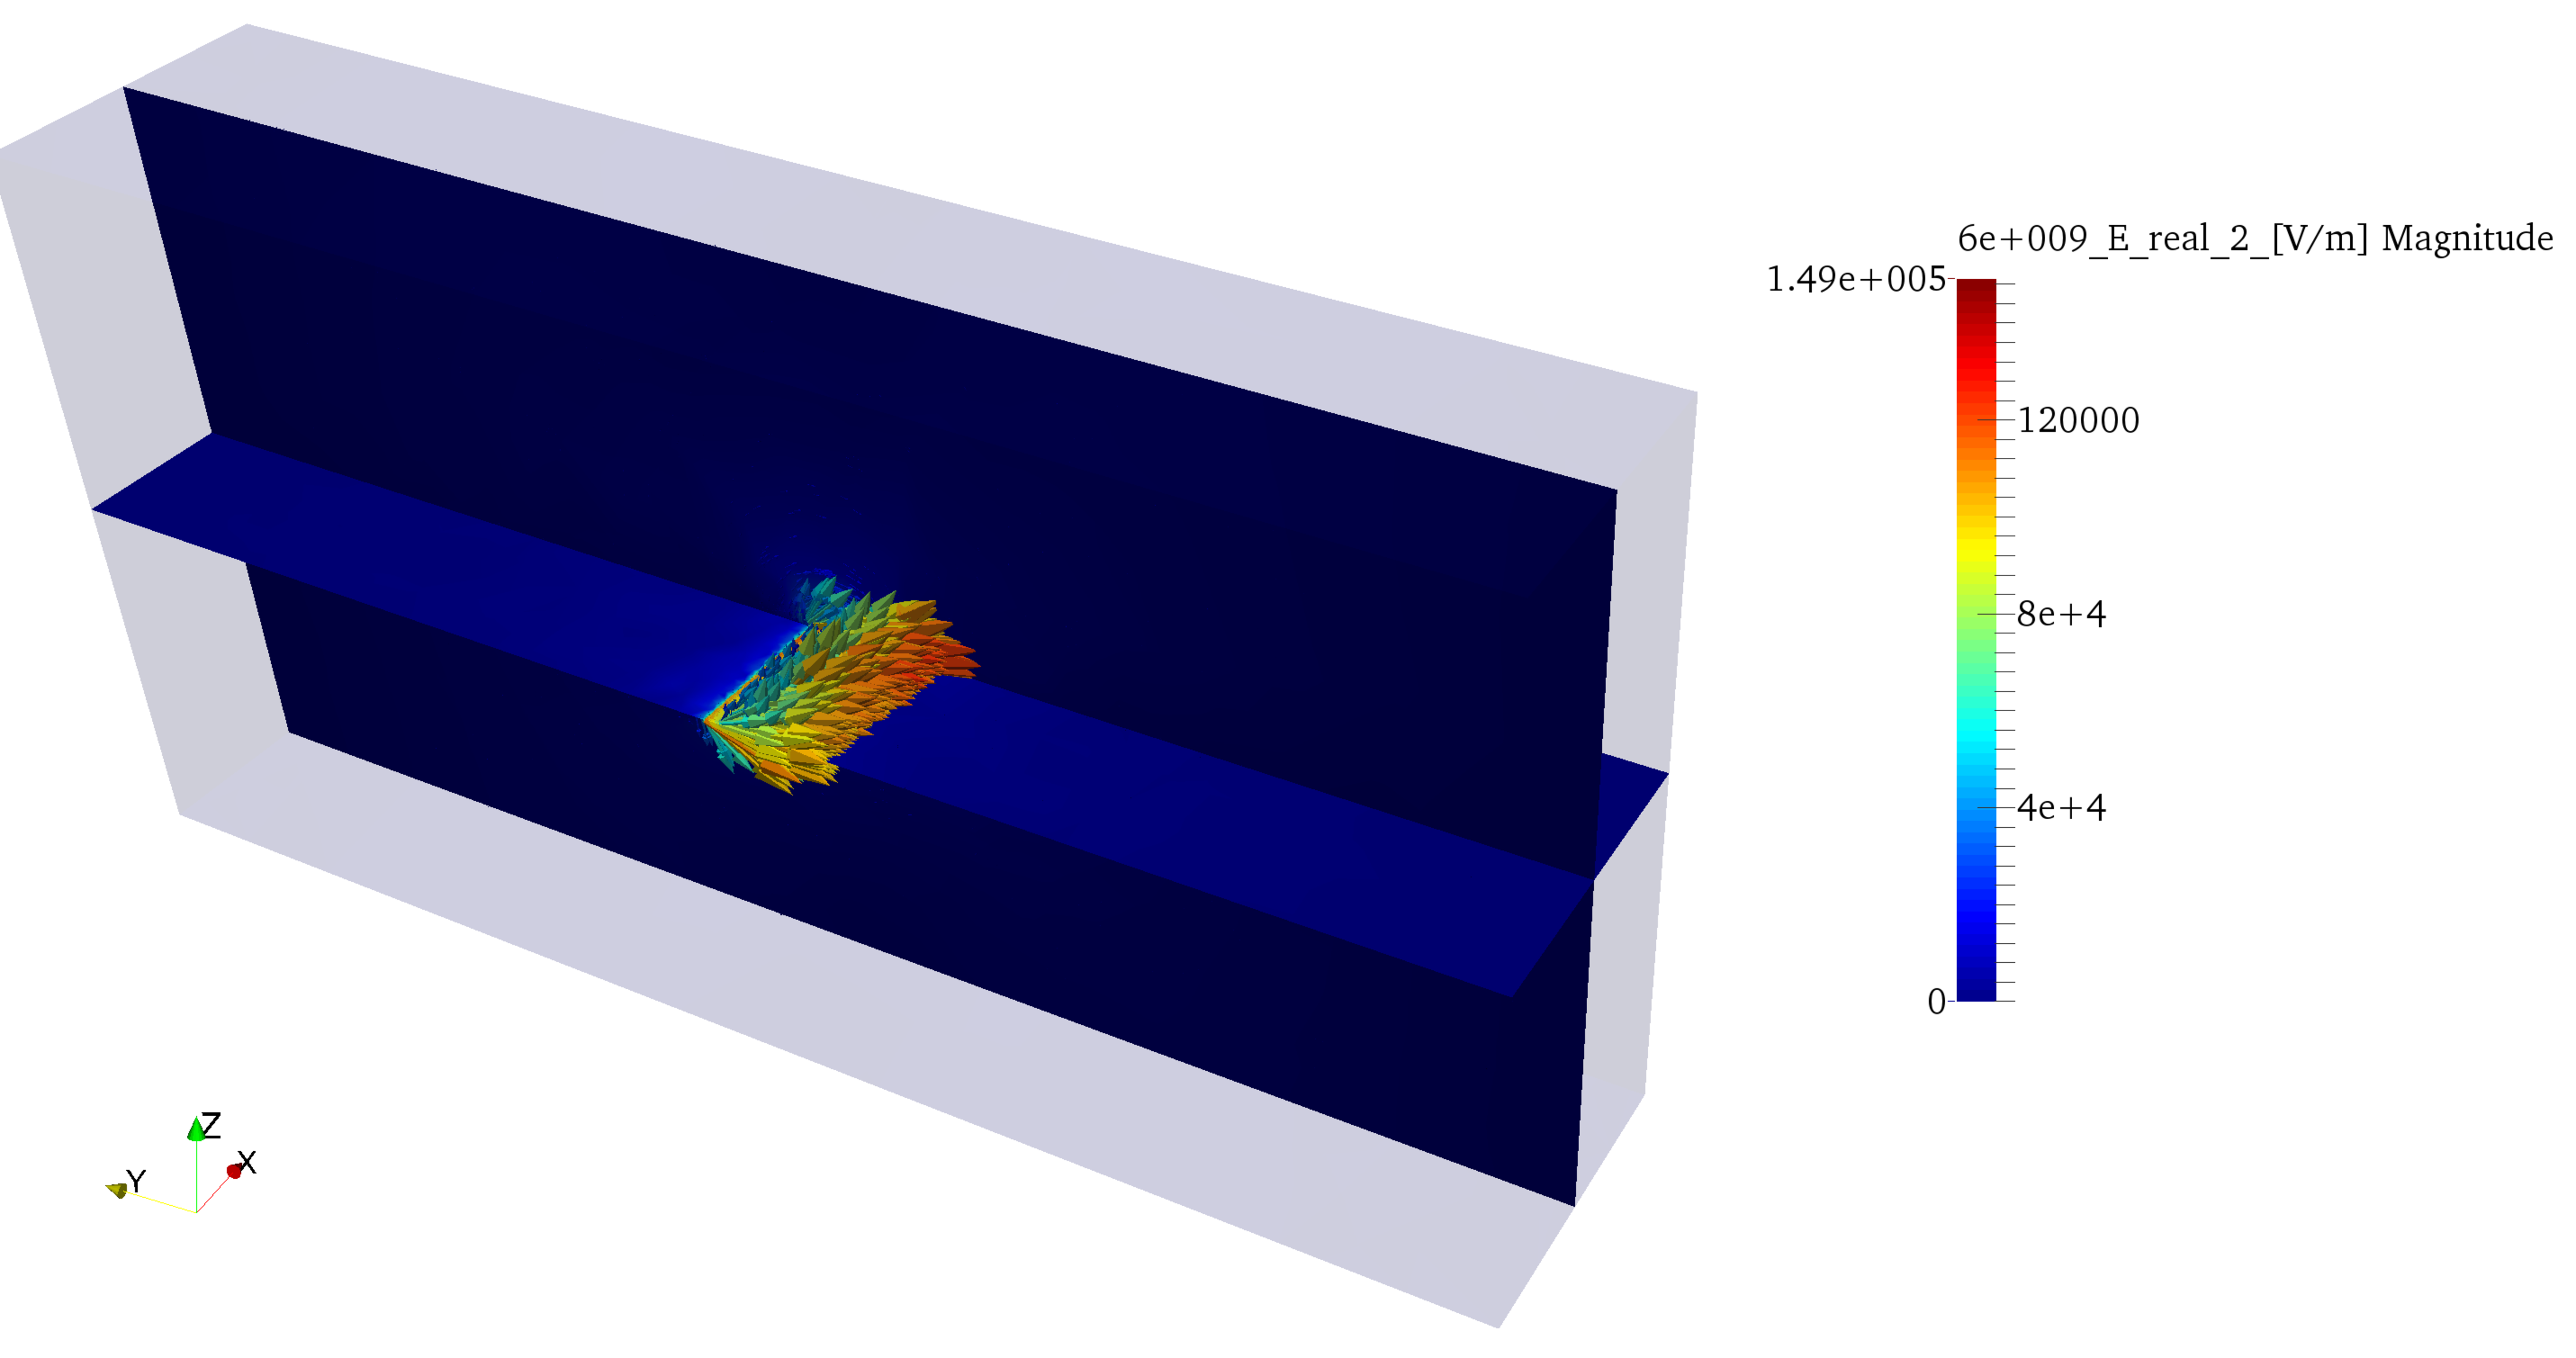
\includegraphics[width=13.4cm]{CPWlin2}
\caption{Stripline mode traveling through the CPW at 6~GHz.}
\label{fig:CPWlin2}
\end{figure}
\begin{figure}[h!]
\centering
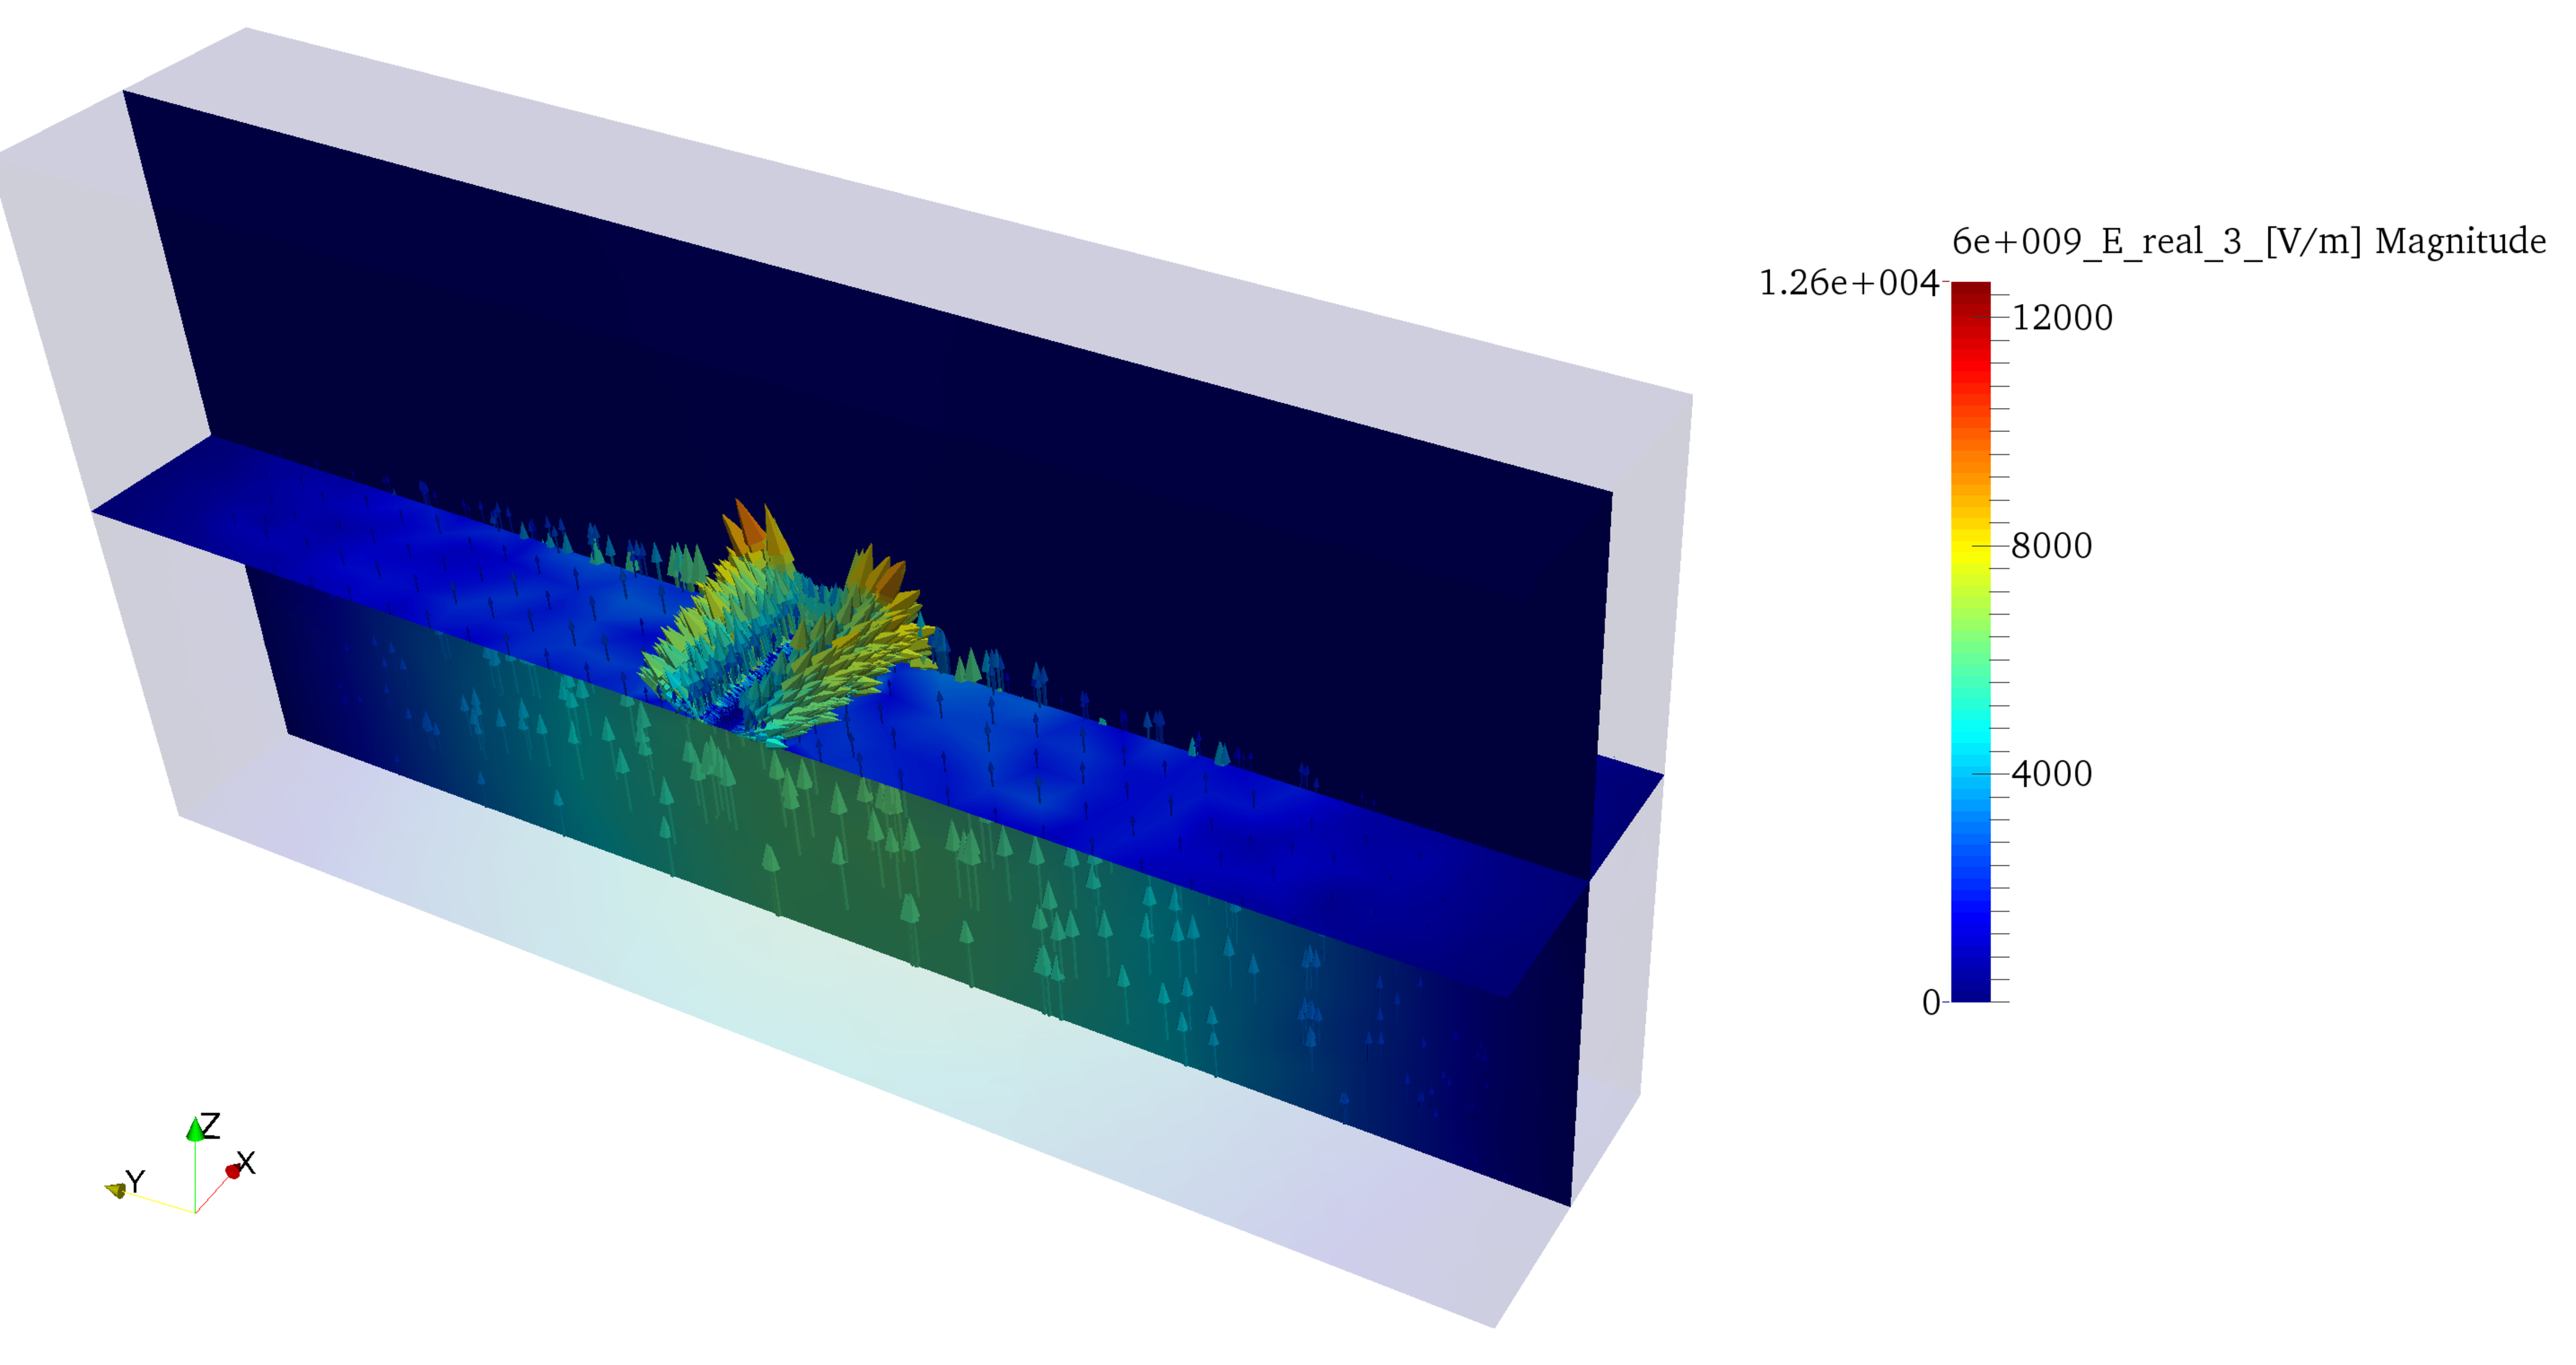
\includegraphics[width=13.4cm]{CPWlin3}
\caption{First hibrid TE mode traveling through the CPW at 6~GHz.}
\label{fig:CPWlin3}
\end{figure}

Finally, the nonlinear analysis is conducted with harmonic orders 1 and 3 ($P=3$) for different impinging powers $\mathrm{P}_1$ at waveport 1: $10^{-3}$, $10^{-2}$, $10^{-1}$, 1, 2, 5 and 10~W of coplanar mode power at 2~GHz. A residual tolerance of $10^{-5}$ as been chosen. The assembly led to 225~798 unknowns and 4 iterations at most were required to tackle the iterative solution for an impinging power of 10~W. The memory and time requirements for each assembly and solve (non-symmetric system) were of 4318~MB and almost 306~s for the slowest iteration. In fact, the first assembled system is almost block diagonal and hence contains less non-zero entries. Only 2335~MB and 267~s were required for the first iteration. The results of the power sweep are shown in Fig. \ref{fig:P3}.
%
\begin{figure}[ht!]
\centering
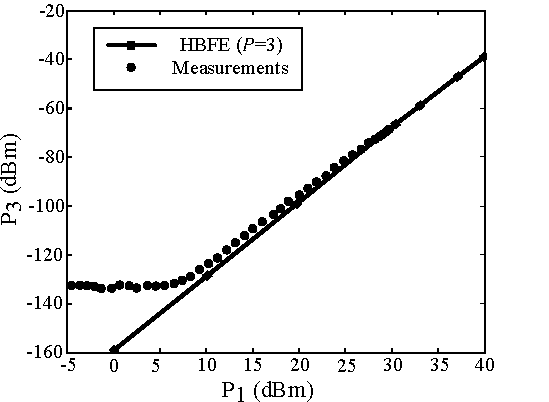
\includegraphics[width=10cm]{P3}
\caption{Third harmonic spurious power computed with the HBFE. Comparisons are with measurements reported in Mateu et al. 2006.}
\label{fig:P3}
\end{figure}
%
The good agreement between the HBFE results, with only $P=3$, and measurements confirms the validity of the method. Fig. \ref{fig:FieldGlyph} shows the total electric field computed contemporaneously at 2~GHz and 6~GHz ($3^\mathrm{rd}$ harmonic).


\begin{figure}[ht!]
\centering
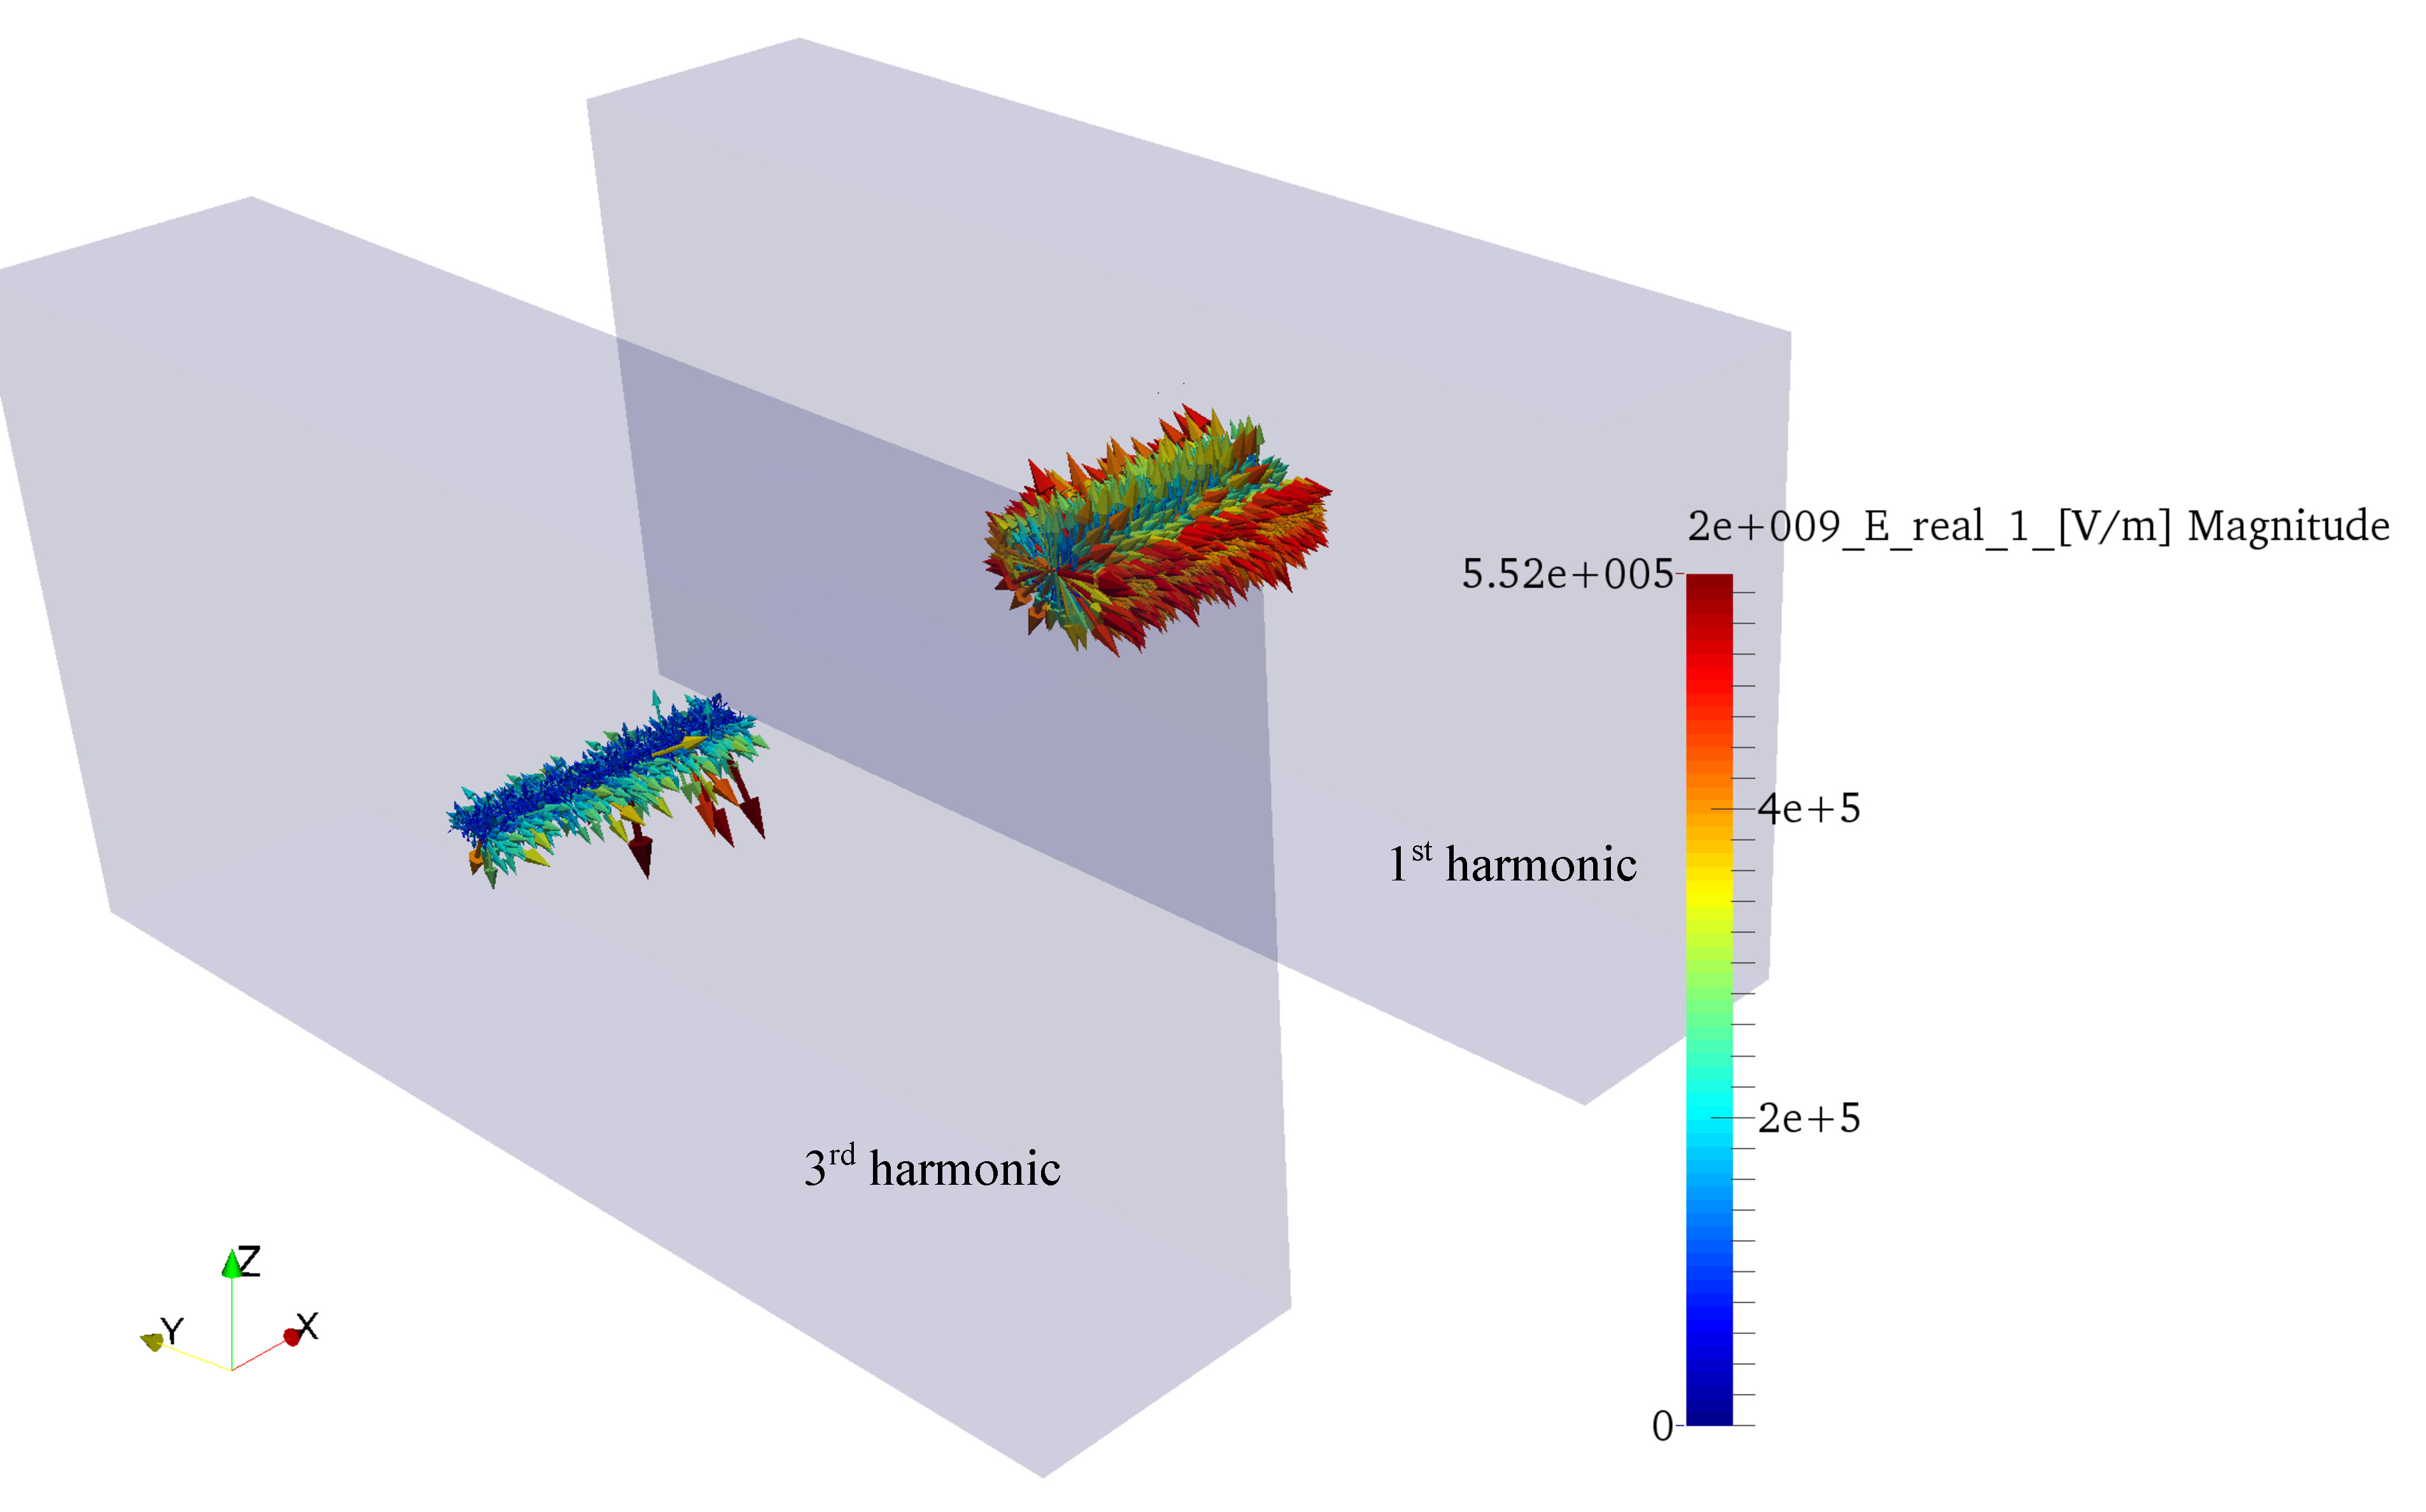
\includegraphics[width=13.4cm]{FieldGlyph}
\caption{Fundamental (2~GHz) and third harmonic electric field distributions computed  by the HBFE with 1~W coplanar mode feeding the CPW.}
\label{fig:FieldGlyph}
\end{figure}

%\begin{figure}[!t]
%\centering
%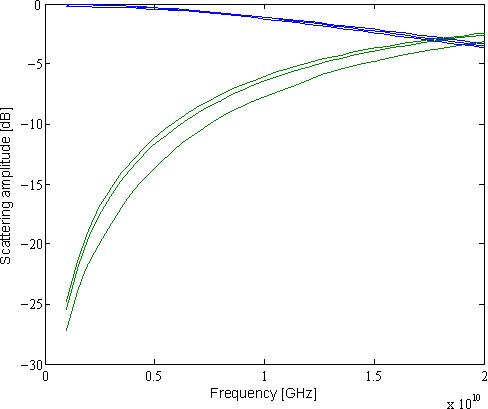
\includegraphics{Gap}
%\caption{}
%\label{fig:P3}
%\end{figure}
